\setcounter{section}{0}
\setcounter{subsection}{0}
\setcounter{subsubsection}{0}
\setcounter{equation}{0}
\pagenumbering{arabic} 
\setcounter{page}{1}    %%%%%KKD used \setcounter{page}{0}  
\oddsidemargin 0.4 cm 
\evensidemargin -.4 cm
%\setlength{\textwidth}{152.4 mm}


\evensidemargin -.2 cm
%\setlength{\textwidth}{152.4 mm}

%\chapter{Synopsis \label{Synopsis}}

{\Large \bf Synopsis}

\newpage

\begin{titlepage}

%\newcommand{\HRule}{\rule{\linewidth}{0.5mm}} % Defines a new command for the horizontal lines, change thickness here
%\newcommand{\eg}{{$\rm e.g.,$ }}
%\newcommand{\cPZ}{{$\rm Z$ }}
%\newcommand{\zll}{{$\rm Z(\ell^{+} \ell^{-})$+jets }}
%\newcommand{\znn}{{$\rm Z(\nu \bar{\nu})$+jets }}
%\newcommand{\gjets}{{ $\rm \gamma$+jets }}

%\newcommand{\nbjets}{{$\rm N_{b-jet}$}}
%\newcommand{\njets}{{$\rm N_{jet}$}}
%\newcommand{\MHT}{{$\rm H_{T}^{miss}$}}
%\newcommand{\HT}{{$\rm H_{T}$}}
%\newcommand{\dphi}{{\rm $\rm \Delta \phi$}}
%\newcommand{\pt}{{$\rm p_{T}$}}

%\end{titlepage}



%\center % Center everything on the page
 

\begin{center}
%\HRule \\[0.4cm]
{ \huge \bfseries Search for Supersymmetry, Leptoquarks and Study of Advanced Pileup Mitigation Techniques}\\[0.4cm] % Title of your document
%\HRule \\[1.5cm]
 
%----------------------------------------------------------------------------------------
%	AUTHOR SECTION
%----------------------------------------------------------------------------------------


\vspace{1cm}
{\bf Bibhuprasad Mahakud}


\vspace{0.5cm}
Department of High Energy Physics

Tata Institute of Fundamental Research,

Homi Bhabha Road, Mumbai 400005, India

\end{center}
%\begin{minipage}{0.2\textwidth}
%\begin{flushleft} \large
%\emph{Author:}\\
%Bibhuprasad \textsc{Mahakud} % Your name
%\end{flushleft}
%\end{minipage}
%~
%\begin{minipage}{0.2\textwidth}
%\begin{flushright} \large
%\emph{Supervisor:} \\
%Prof. Gagan \textsc{Mohanty} % Supervisor's Name
%\end{flushright}
%\end{minipage}\\[1cm]

\vspace{1.5cm}

%\begin{abstract}

We search for supersymmetry in all hadronic final states with proton-proton collision data recorded by the CMS detector at a center-of-mass energy of 13 TeV. We specifically target for pair produced gluinos in the 2015 data that correspond to an integrated luminosity of $\rm 2.3 fb^{-1}$, and using more than five times  data collected during 2016 where we also add stop and other squark pairs to our search. The data are examined in search regions of jet multiplicity, tagged bottom quark jet multiplicity, missing transverse momentum, and the scalar sum of jet transverse momenta. The observed numbers of events in all search regions are found to be consistent with the expectations from standard model processes. Exclusion limits are calculated for simplified supersymmetric models of gluino pair production. Depending on the assumed gluino decay mechanism, and for a massless, weakly interacting, lightest neutralino, lower limits on the gluino mass from 1440 to 1700 GeV are obtained, significantly extending previous limits.

Another search for the pair production of first generation scalar leptoquarks decaying to leptons and jets is presented. The data corresponding to 2.6 $\rm fb^{-1}$ were collected from proton-proton collisions at a center-of-mass energy of 13 TeV. No significant deviation is found with respect to the standard model predictions. Upper limits are set on cross section times branching fraction.  

The increase of instantaneous luminosity for Run II LHC results in a large number of additional proton-proton collisions in a given event (pileup) leading to contamination of jets. We study advanced pileup removal techniques like trimming, pruning and soft-drop  etc. The focus was on preparation for Run II for which we expected up to 40 additional pileup events in comparison to Run I LHC data that had typically half the pileup events on average.


%\end{abstract}
%~\cite{JMEPAS}
%~\cite{LQPAS}

\vspace{1cm}

\begin{center}
{\bf Advisor: Prof. Gagan B. Mohanty}
\end{center}


\newpage

\bf{\LARGE List of Publications}

\vspace{2cm}
\underline{\bf \Large{Journals}}

\begin{itemize}

\item {\bf  Search for supersymmetry in the multijet and missing transverse momentum final state in pp collisions at 13 TeV, \textcolor{blue}{Phys. Lett. B 758 (2016) 152}.}
%\vspace{1cm}

\end{itemize}
\vspace{0.5cm}
\underline{\bf \Large{CMS Physics Analysis Summary (Public Results)}}

\begin{itemize}
\item {\bf Search for supersymmetry in events with jets and missing
transverse momentum in proton-proton collisions at 13 TeV, \textcolor{blue}{CMS-PAS-SUS-16-014}.}

\item{\bf Search for supersymmetry in the multijet and missing transverse momentum channel in pp collisions at 13 TeV, \textcolor{blue}{CMS-PAS-SUS-15-002}. }

\item{\bf Search for pair-production of first generation scalar leptoquarks in pp collisions at $\rm \sqrt{s}$=13 TeV with 2.6 $\rm fb^{-1}$, \textcolor{blue}{CMS-PAS-EXO-16-043}. }

\item{\bf Study of Pileup Removal Algorithms for Jets, \textcolor{blue}{CMS-PAS-JME-14-001}.}

\end{itemize}
\vspace{0.5cm}
\underline{\bf \Large{Conference Proceedings}}

\begin{itemize}

\item {\bf Search for SUSY in jets+MET final state, \textcolor{blue}{ PoS(DIS2016)094}.}

\end{itemize}
\vspace{0.5cm}
\underline{\bf \Large{CMS Internal Notes}}

\begin{itemize}

\item {\bf Search for supersymmetry in multijet final states in proton-proton collisions at 13 TeV, \textcolor{blue}{CMS-AN-16-188}.}

\item{\bf Search for supersymmetry in the multijet and missing transverse momentum channel in pp collisions at 13 TeV, \textcolor{blue}{CMS-AN-15-003}. }

\item{\bf Search for Pair-production of Scalar First Generation
Leptoquarks in pp Collisions at $\sqrt{s}$ = 13 TeV, \textcolor{blue}{CMS-AN-15-294}. }

\item{\bf Study of Pileup Removal Algorithms for Jets, \textcolor{blue}{CMS-AN-14-175}.}

\end{itemize}

%\textsc{\large Tata institute of fundamental research , Mumbai}\\[0.5cm] % Minor heading such as course title
% If you don't want a supervisor, uncomment the two lines below and remove the section above
%\Large \emph{Author:}\\
%John \textsc{Smith}\\[3cm] % Your name

%----------------------------------------------------------------------------------------
%	DATE SECTION
%----------------------------------------------------------------------------------------

%{\large \today}\\[1cm] % Date, change the \today to a set date if you want to be precise

%----------------------------------------------------------------------------------------
%	LOGO SECTION
%----------------------------------------------------------------------------------------

%
\includegraphics{TIFRlogo.png}\\[0.5cm] % Include a department/university logo - this will require the graphicx package
 
%----------------------------------------------------------------------------------------

\vfill % Fill the rest of the page with whitespace

\end{titlepage}

%\tableofcontents


\newpage



\section{Introduction}

The standard model (SM) of particle physics successfully describes a wide range of phenomena.
However, it is unable to explain the stability of the Higgs boson mass in the face of higher-order corrections, suggesting
that the model is incomplete. Many extensions to the SM have been proposed to provide a more
fundamental theory.  Supersymmetry (SUSY)~\cite{SUSYtheo}, one such extension, postulates that each
SM particle has a SUSY partner from which it differs in spin by half a unit.  As
examples, squarks and gluinos are the SUSY partners of quarks and gluons, respectively, while
neutralinos arise from a mixture of the SUSY partners of neutral (charged)
Higgs and electroweak gauge bosons. Radiative corrections involving SUSY particles can compensate the contributions from SM particles and thereby stabilize the Higgs boson mass.  For this cancellation to be natural, the top and bottom squark, and gluino must have
masses on the order of a few TeVs, possibly allowing them to be produced at the CERN
LHC.

Amongst SUSY processes,  the gluino pair production,  typically yielding four or more hadronic
jets in the final state, has the largest possible cross section, making it an apt channel at
 the recently started LHC Run 2. In R-parity ~\cite{RParity} conserving
SUSY models, as are considered here, the lightest SUSY particle (LSP) is stable and assumed
to be weakly interacting, leading to potentially large undetected, or missing, transverse momentum. Supersymmetry events at the LHC might thus be characterized by significant missing
transverse momentum, numerous jets, and in the context of natural SUSY ~\cite{Naturaln}, jets initiated
by top and bottom quarks.

In this search, we consider SUSY scenarios in the context of simplified models~\cite{SMS1} of new particle
production. Diagrams for the three models are shown in Fig. 1. Simplified models contain
the minimal particle content to represent a topological configuration. As for SUSY production
scenarios, the four simplified models can be interpreted as follows. In the first one, shown
in Fig. 1 (left), the gluino pair production is followed by the decay of each gluino to a bottom
quark and an off-shell bottom squark. The off-shell bottom squark decays to a bottom quark
and the LSP, where the LSP is assumed to be the lightest neutralino 
that escapes detection, leading to significant missing transverse energy. The second scenario, shown in Fig. 1 (middle), is the same as the first one except with top quarks and off-shell top squarks appearing in place of the bottom
quarks and squarks. The third scenario, shown in Fig. 1 (right), is the corresponding
situation with the gluino decay to a light-flavored quark and off-shell squark up, down, strange,
and charm with equal probability, for each of them separately separately. 

\begin{figure}[h]
\centering
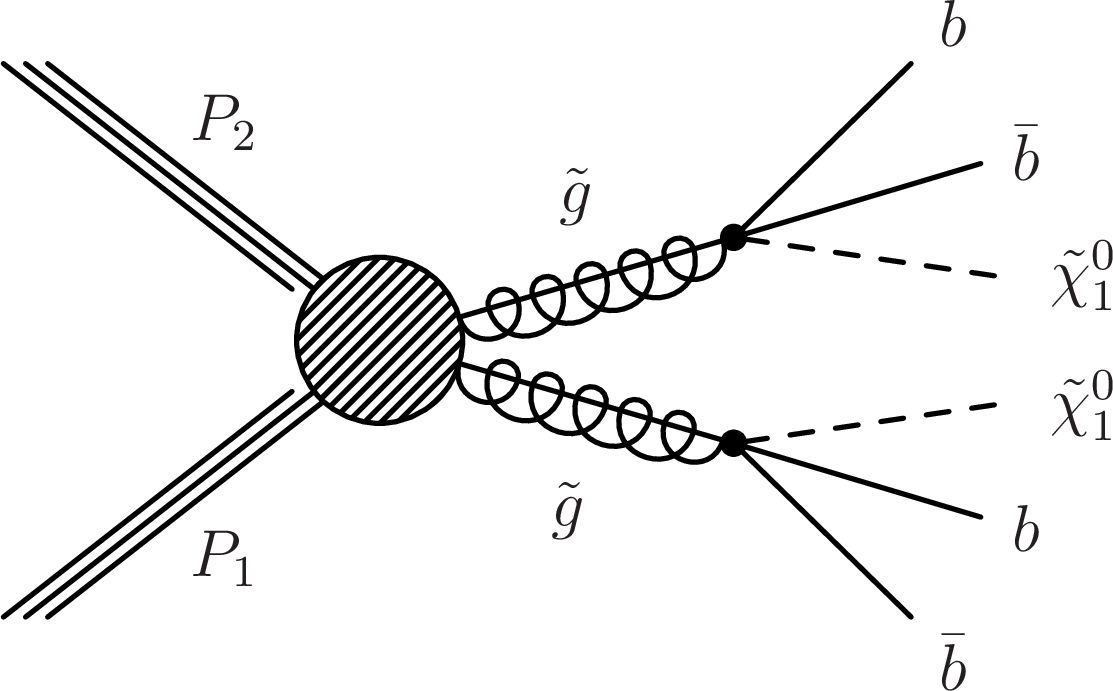
\includegraphics[width=0.3\textwidth]{/home/bibhu/Desktop/PhDThesis/PhDThesis/synopsis/T1bbbb.png}
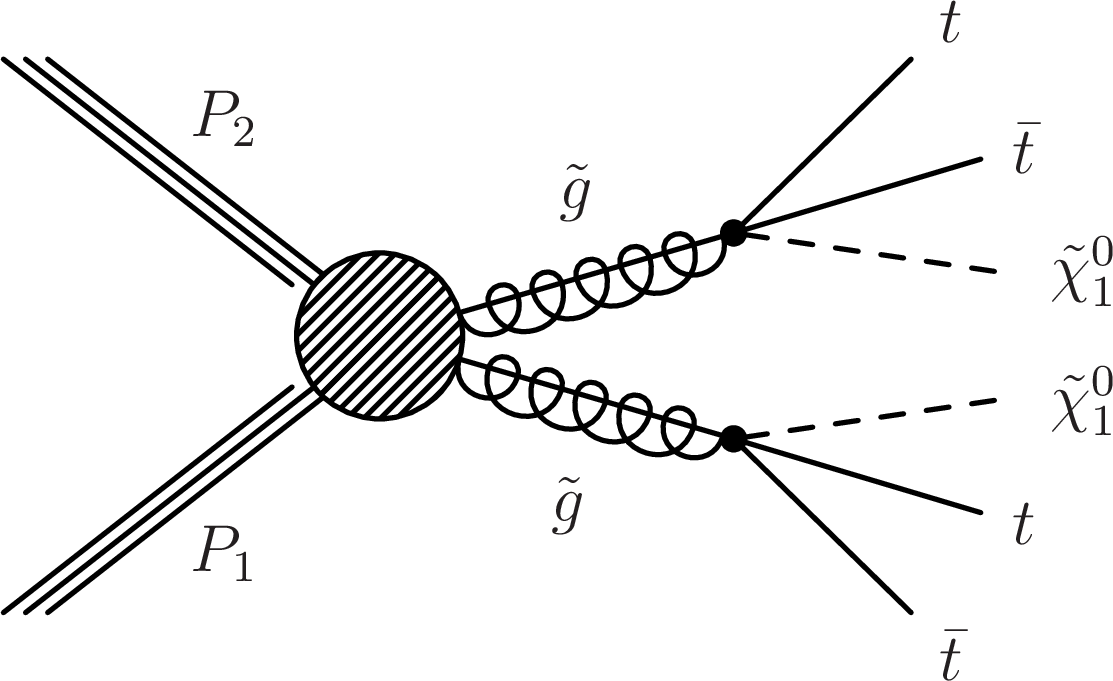
\includegraphics[width=0.3\textwidth]{/home/bibhu/Desktop/PhDThesis/PhDThesis/synopsis/T1tttt.png}
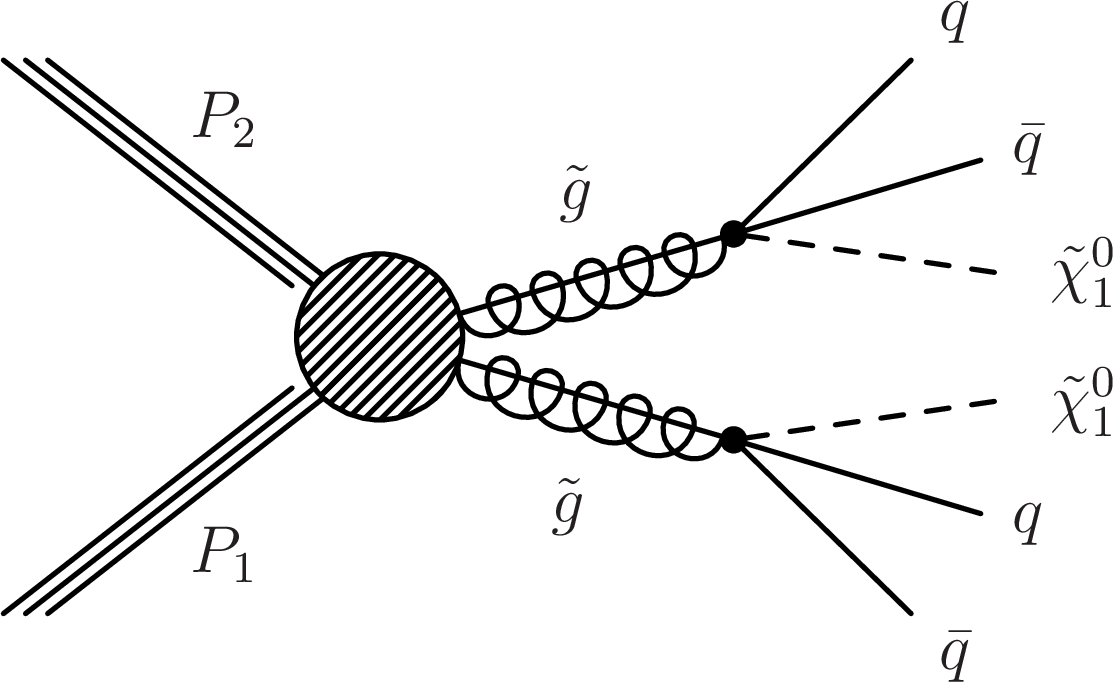
\includegraphics[width=0.3\textwidth]{/home/bibhu/Desktop/PhDThesis/PhDThesis/synopsis/T1qqqq.png}

\caption{\label{fig:frog}Event diagrams for the main new-physics scenarios considered in this study.}
\end{figure}

The SM quark and lepton sectors are strikingly similar in terms of the number of particles and generations. This hints that the two sectors could be
related by a fundamental symmetry. Many beyond the SM theories, include
such a symmetry~\cite{composite,LQ2,LQ3,LQ4}, which gives rise to new class of bosons called leptoquarks (LQs). LQs couple
to both leptons and quarks, carrying lepton and baryon numbers as well as fractional electric charge.
They can be either scalar or vector particles (carrying zero or one unit of spin) and are color
triplets. Current experimental searches for rare processes mediated by lepton number violation and
flavor-changing neutral currents suggest that LQs come in three generations which do
not mix. Their pair-production at the LHC proceeds mainly via gluon-gluon (gg) fusion  and
quark-antiquark ($\rm q\bar{q}$) annihilation. Due  to  the gg dominance,  along  with  the  fact  that  only  one q-Feynman  diagram
contains the LQ-quark-lepton vertex, the scalar LQ pair-production has a negligible dependence on the
 LQ-quark-lepton Yukawa coupling, usually denoted as $\lambda$. LQ searches are essentially independent of $\lambda$. 
In our search we consider pair produced LQs with each of them decaying to an electron and a quark. Therefore we look for signature in two electron and two jet final states in the data.

In the two physics topics discussed above as well as many other important studies at the LHC, the performance of jets is extremely important.
 One of the key challenges of the  LHC run is the increase of instantaneous luminosity, which results in a large number of additional proton-proton collisions (pileup) in each event. In such high pileup environment, an accurate reconstruction of jet properties and shapes has become more and more demanding. The most common observables for jets at the LHC  are primarily the jet $\rm p_{T}$, pseudorapidity($\eta$), and $\phi$.
In recent years, it is becoming increasingly popular to consider the internal structure of the jet. The applications include the discrimination of quark- and gluon-initiated jets as well as the identification of highly boosted hadronically decaying heavy resonances such as W/Z or Higgs boson that are contained in a single jet.  
In all such cases, contamination from pileup degrades our ability to effectively reconstruct the jet observables.  
Motivated by this, we study advanced techniques for pileup mitigation for jets in view of high pileup scenarios in Run II of the LHC.





\section{CMS Detector }
The CMS detector is built around a superconducting solenoid of 6-m internal diameter, providing
a magnetic field of 3.8 T. Within the solenoid volume are a silicon pixel and microstrip tracker, a
lead tungstate crystal electromagnetic calorimeter (ECAL), and a brass-scintillator sandwich hadron
calorimeter (HCAL). The tracking detectors cover a range of  $|\eta|$ $<$  2.5. The ECAL and HCAL, each composed of a barrel and two endcap sections, extend over  $|\eta|$ $<$ 3.0. Forward calorimeters on either side of the
interaction point encompass 3.0 $<$  $|\eta|$ $<$ 5.0. Muons
are measured within $|\eta|$ $<$ 2.4 by gas-ionization detectors embedded in the steel flux-return
yoke outside the solenoid. The detector is nearly hermetic, permitting accurate measurements
of missing transverse energy. A more detailed description of the detector, together with a definition of the
coordinate system and relevant kinematic variables, is given in Ref.~\cite{cms}. The studies presented in the thesis use information from all parts of the CMS detector.

\section{Event Reconstruction }
Physics objects used in our studies are defined using the so-called particle flow (PF) algorithm ~\cite{Beaudette:2014cea}, which reconstructs
and identifies individual particles through an optimized combination of information from different
detector components. The PF candidates are classified as photons, charged and
neutral hadrons, electrons, or muons. Additional quality criteria are imposed on electron,
muon and photon candidates. For example, more restrictive conditions are placed on the
shower shape and on the ratio of energies deposited in the HCAL and ECAL for electron and photon candidates,
and similarly on the matching of track segments between the silicon tracker and muon detector
for muon candidates. Photons being neutral particles do not produce tracks in the tracker, while electrons do. The event primary vertex is taken to be the one reconstructed with the
largest sum of charged-track $\rm p_{T}^{2}$ values and is required to lie within 24 cm (2 cm) of the center of
the detector in the direction along (perpendicular to) the beam axis. Tracks from extraneous
pp interactions within the same or a nearby bunch crossing (pileup) are removed .
The PF objects serve as inputs for jet reconstruction, based on the anti-$k_{t}$ algorithm ~\cite{Cacciari:2008gp}  with
a distance parameter of 0.4. Jet quality criteria are applied to eliminate,
for example, spurious events caused by calorimetric noise. Contributions to an individual jet’s
$\rm p_{T}$ from pileup interactions are subtracted, and corrections are applied as a function of jet
$\rm p_{T}$ and $\eta$ to account for residual effects of nonuniform detector response.

\section{ Search for Supersymmetry with 13 TeV pp Collision Data}




Because of the large mass scale and their all-hadronic nature, the targeted SUSY events are expected to exhibit large values of $\rm H_{T}$,
where $\rm H_{T}$ is the scalar sum of the jet $\rm p_{T}$. As a measure of missing
transverse momentum, we use the variable $\rm H_{T}^{miss}$, which is the magnitude of the vector sum of
the jet $\rm p_{T}$. We present a general search for gluino pair production leading to final states with
large $\rm H_{T}$, large $\rm H_{T}^{miss}$ as well as large jet multiplicity. The data are examined in exclusive bins of $ \rm \bf{ N_{jet}}$, $ \rm \bf{ N_{b-jet}}$, $ \rm \bf{ H_{T}}$,
and $ \rm \bf{H_{T}^{miss}}$, where $\rm N_{jet}$ is the number of jets and $\rm N_{b-jet}$, the number of tagged bottom quark jets. 


The principal sources of background arise from the SM production of top quarks, a W or Z
boson in association with jets (W+jets or Z+jets ), and multiple jets through the strong
interaction. We refer to the last class of background as quantum chromodynamics (QCD)
multijet events. Although events with top quarks mostly come from top quark-antiquark ($\rm t\bar{t}$) production,
a modest contribution is also from single top quark processes. The W and Z bosons in W+jets and Z+jets events
can be either on- or off-shell. For top quark and W+jets events, significant $\rm H_{T}^{miss}$  can arise if the
W boson decays leptonically, producing a neutrino and an undetected charged lepton, while
Z+jets events can exhibit significant $\rm H_{T}^{miss}$ if the Z boson decays to two neutrinos. For QCD
multijet events, significant $\rm H_{T}^{miss}$ can arise if the event contains a charm or bottom quark that
undergoes a semileptonic decay; however the principal source is the mismeasurement of
jet $\rm p_{T}$. The signal vs. background composition plots in search variables are shown in Fig.~\ref{fig:SigvsBkgSearchVariables1Synop} and ~\ref{fig:SigvsBkgSearchVariables2Synop}.

\begin{figure}[h]
\begin{center}
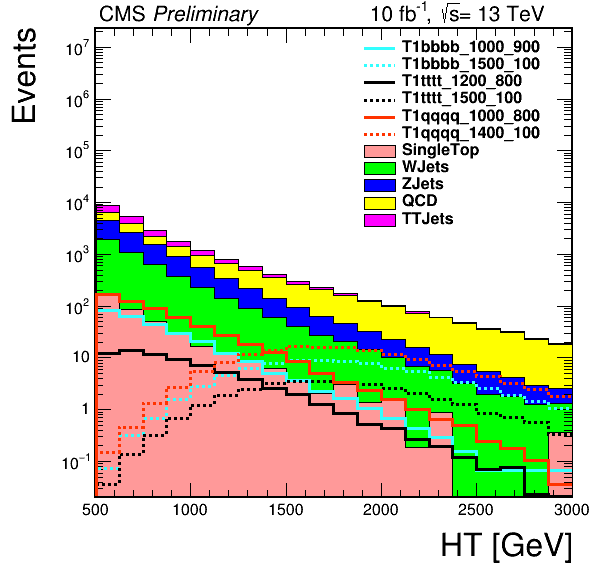
\includegraphics[width=0.35\textwidth]{/home/bibhu/Desktop/PhDThesis/PhDThesis/synopsis/HT_distribution.png}
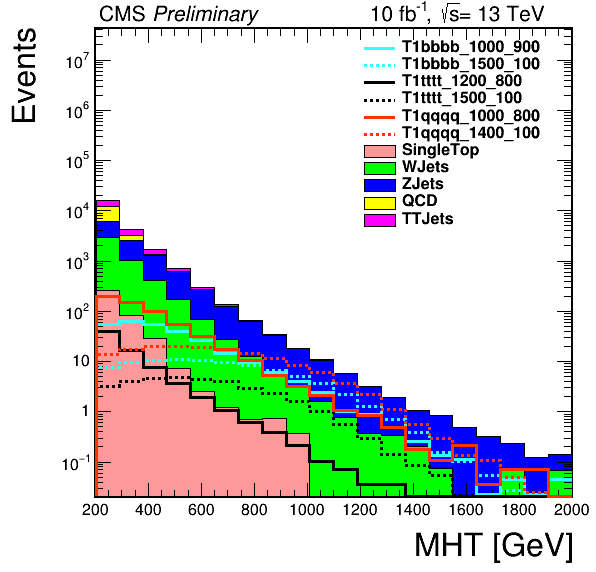
\includegraphics[width=0.35\textwidth]{/home/bibhu/Desktop/PhDThesis/PhDThesis/synopsis/MHT_distribution.png}
\caption{\label{fig:SigvsBkgSearchVariables1Synop} Signal vs. stacked backgrounds in $\rm H_{T}$($~$HT, left) and $\rm H_{T}^{miss}$($~$MHT, right)}
\end{center}
\end{figure}

\begin{figure}[h]
\begin{center}
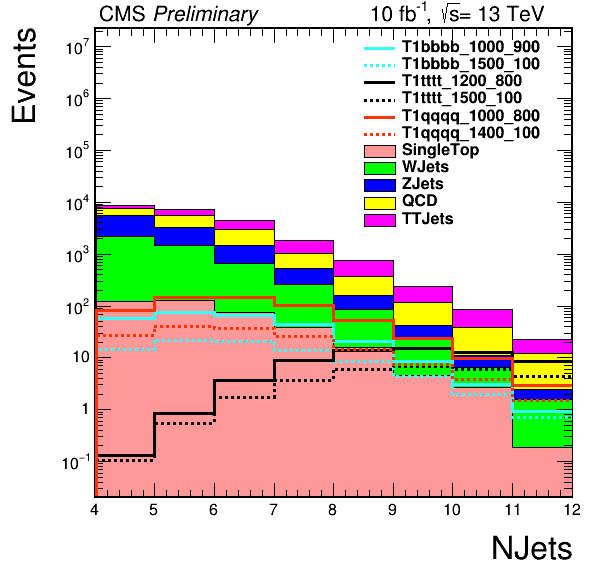
\includegraphics[width=0.35\textwidth]{/home/bibhu/Desktop/PhDThesis/PhDThesis/synopsis/NJets_distribution.png}
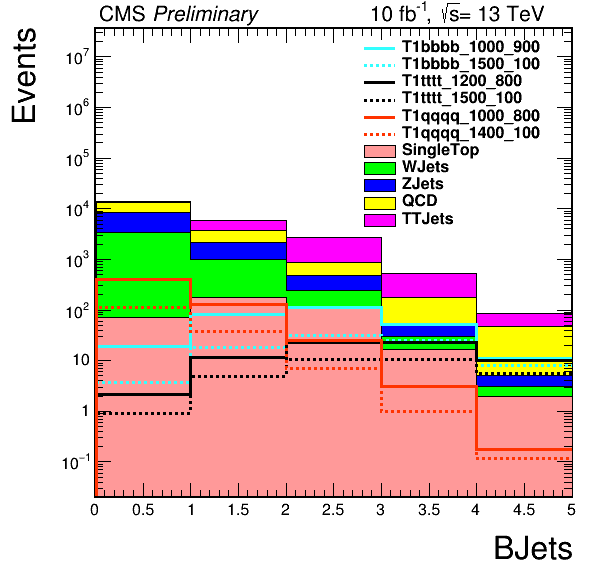
\includegraphics[width=0.35\textwidth]{/home/bibhu/Desktop/PhDThesis/PhDThesis/synopsis/BJets_distribution.png}
\caption{\label{fig:SigvsBkgSearchVariables2Synop} Signal vs. stacked backgrounds in $\rm N_{jet}$(NJets, left) and $\rm N_{b-jet}$(MHT, right)}
\end{center}
\end{figure}


\subsection{Study on 2.3 $\rm fb^{-1}$ of 2015 Data}

In this section, we discuss the analysis strategy and results of the search conducted using 2015 data. With as little as 
2.3 $\rm fb^{-1}$ data we search for gluino pair production based on the above four variables. To get maximum signal and minimum background we select events with the criteria defined below.

\subsubsection{Event Selection and Search Region}  
The following requirements define the  signal event candidates:
\begin{itemize}
\item $\rm N_{jet}$ $\geq$ 4, where the jets must lie within $|\eta|$ $<$ 2.4; we require at least four jets because of
our focus on gluino pair production;
\item $\rm H_{T}$ $\textgreater $ 500 GeV, where $\rm H_{T}$ is the scalar $\rm p_{T}$ sum of jets with $|\eta|$ $<$ 2.4;

\item $\rm H_{T}^{miss}$ $>$ 200 GeV, where $\rm H_{T}^{miss}$ is the magnitude of $\rm \overrightarrow{H}_{T}^{miss}$, the negative of the vector
$\rm p_{T}$ sum of jets with $|\eta|$ $<$ 5; the $\eta$ range is extended in this case so that  ${\rm \overrightarrow{H}_{T}^{miss}}$ better
represents the total missing transverse momentum in a given event;

\item  No identified, isolated electron (muon) candidate with $\rm p_{T}$ $\textgreater$ 10 GeV and $|\eta|$ $<$ 2.5 ($<$2.4);

\item No isolated charged-particle track with $|\eta|$ $<$  2.4, $\rm m_{T}$ $<$ 100 GeV, and $\rm p_{T}$ $\textgreater $ 10 GeV
($p_{T}$ $\textgreater$ 5 GeV if the track is identified as an electron or muon candidate) where $\rm m_{T}$ is the transverse mass formed from the ${\rm \overrightarrow{p_{T}}^{miss}}$ and isolated-track
$\rm p_{T}$ vector, with ${\rm \overrightarrow{H}_{T}^{miss}}$ the negative of the vector  $\rm p_{T}$ sum of all PF objects;

\item  $\Delta \phi_{\rm \overrightarrow{H}_{T}^{miss},j_{i}}$  $\textgreater$ 0.5 ($\textgreater$0.3) for the two highest $\rm p_{T}$ jets $\rm j_{1}$ and $\rm j_{2}$ (the next two highest $\rm p_{T}$ jets
$\rm j_{3}$ and $\rm j_{4}$), with   the azimuthal angle between $\rm H_{T}^{miss}$ and the $\rm p_{T}$ vector of jet $\rm j_{i}$.

\end{itemize}
The search is performed in the following 72 ($=3\times4\times3\times3$) exclusive intervals of the four search variables:
\begin{itemize}

 \item ${\bf 3 }$ $\rm N_{jet}$ bins: 4-6, 7-8 and $\geq$9;
 \item ${\bf 4 }$ $\rm N_{b-jet}$ bins: 0, 1, 2 and $\geq$3;
 \item ${\bf 3 }$ $\rm H_{T}$ bins: 500-800, 800-1200 and $\textgreater$1200 GeV;
 \item ${\bf 3 }$ $\rm H_{T}^{miss}$ bins : 200-500, 500-750 and $\textgreater$750 GeV.
\end{itemize}

\subsubsection{Background Estimation }
In this section, we describe the evaluation of the background from SM processes. The evaluation
relies on data control regions (CRs) selected using similar criteria to the search regions. The backgrounds are 
divided into four different types, namely Z to neutrinos, lost lepton, QCD and hadronic tau.

\paragraph{\underline {Z to neutrinos}: }


This is the most important backgrounds being an irreducible one. We are talking about events with a Z boson produced in association with jets when the Z decays to two neutrinos. The most straightforward way to measure this background is
to exploit the decays $\rm Z(\ell^{+} \ell^{-})$+jets in which the Z boson can be
reconstructed from the observed pair of muons or electrons.  The
efficiency-corrected yields from these decays can be translated
directly into the $\rm Z(\nu \bar{\nu})$+jets background yield by the known branching
ratios.  The limitation of this approach arises from the rather small
branching ratio between the charged and neutral leptons, so that the
transfer factor from the control sample measurement to the predicted
background is larger than one (ignoring efficiencies, the
branching ratio itself is approximately 3 when both muon and electron
pairs are used). 

The alternative approach is to exploit the similarity to Z boson
radiation of the more copious radiation of photons.  Here the
challenge is to obtain validation in data of the MC predictions
connecting the two processes.

Our baseline strategy is to use the $\rm \gamma$+jets sample to determine the
yields in the 18 bins corresponding to $\rm N_{b-jet}$=0.  These are
compared with the $\rm Z(\ell^{+} \ell^{-})$+jets yields in the low-$\rm N_{jet}$
bin to establish the systematic uncertainty of the physics modeling of
$\rm \gamma$+jets, and the normalization corrected if necessary.  
The extrapolation to bins with $\rm N_{b-jet}>$0 is performed to
the extent possible with the $\rm Z(\ell^{+} \ell^{-})$+jets data sample, supplemented with MC
information where necessary. We use simulation to correct for the
resulting distribution to the higher $\rm N_{jet}$ bins.

As shown in Eq.(~\ref{eq:gjet1}), we predict the number of $\rm Z(\to\nu \bar{\nu})$+jets events contributing 
to each of the 18 0-btag analysis bins ($\rm N_{Z(\to\nu \bar{\nu})}^{\rm pred}$) from the number of events in the corresponding 
bin of the $\gamma$+jets control sample ($\rm N_{\gamma}^{\rm obs}$), the purity of the 
control sample ($\beta$), and the ratio of the numbers of $\rm Z\to\nu \bar{\nu}$+jets events and $\gamma$+jets events 
obtained from leading order {\sc MadGraph}+{\sc Pythia} (${\cal
  R}_{Z(\nu\bar{\nu})/\gamma} \cdot {\cal F}_{\rm dir}$).  Here ${\cal
  F}_{\rm dir}$ is the fraction of prompt photons that are direct.
\begin{align}
N_{Z\to\nu \bar{\nu}}^{\rm pred} &= DR\cdot {\cal R}_{Z(\nu\bar{\nu})/\gamma} \cdot {\cal F}_{\rm dir} \cdot \beta \cdot N_{\gamma}^{\rm obs}
\label{eq:gjet1}
\end{align}

\begin{figure}
\begin{center}
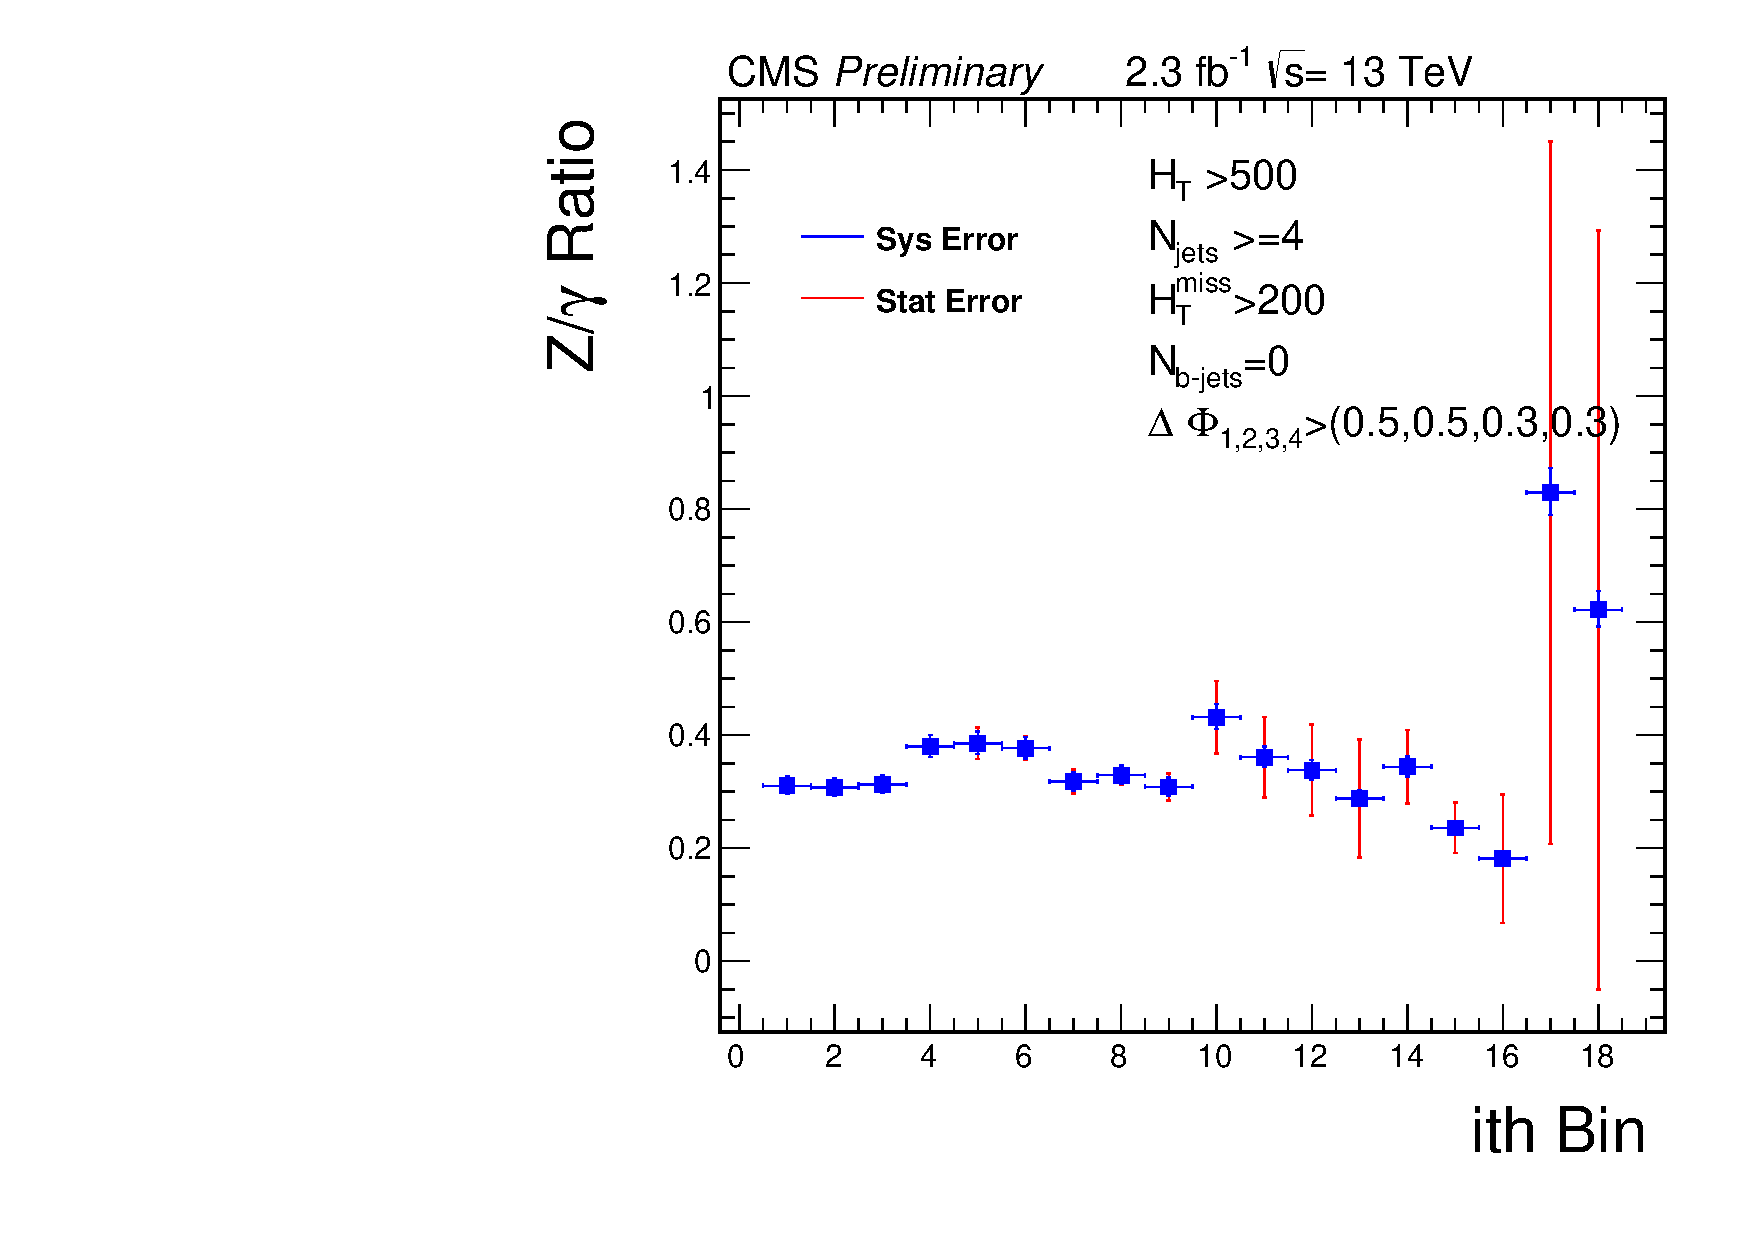
\includegraphics[width=0.35\textwidth]{/home/bibhu/Desktop/PhDThesis/PhDThesis/synopsis/ZGammaRatioWSF.pdf} % ADDNEWPLOT 
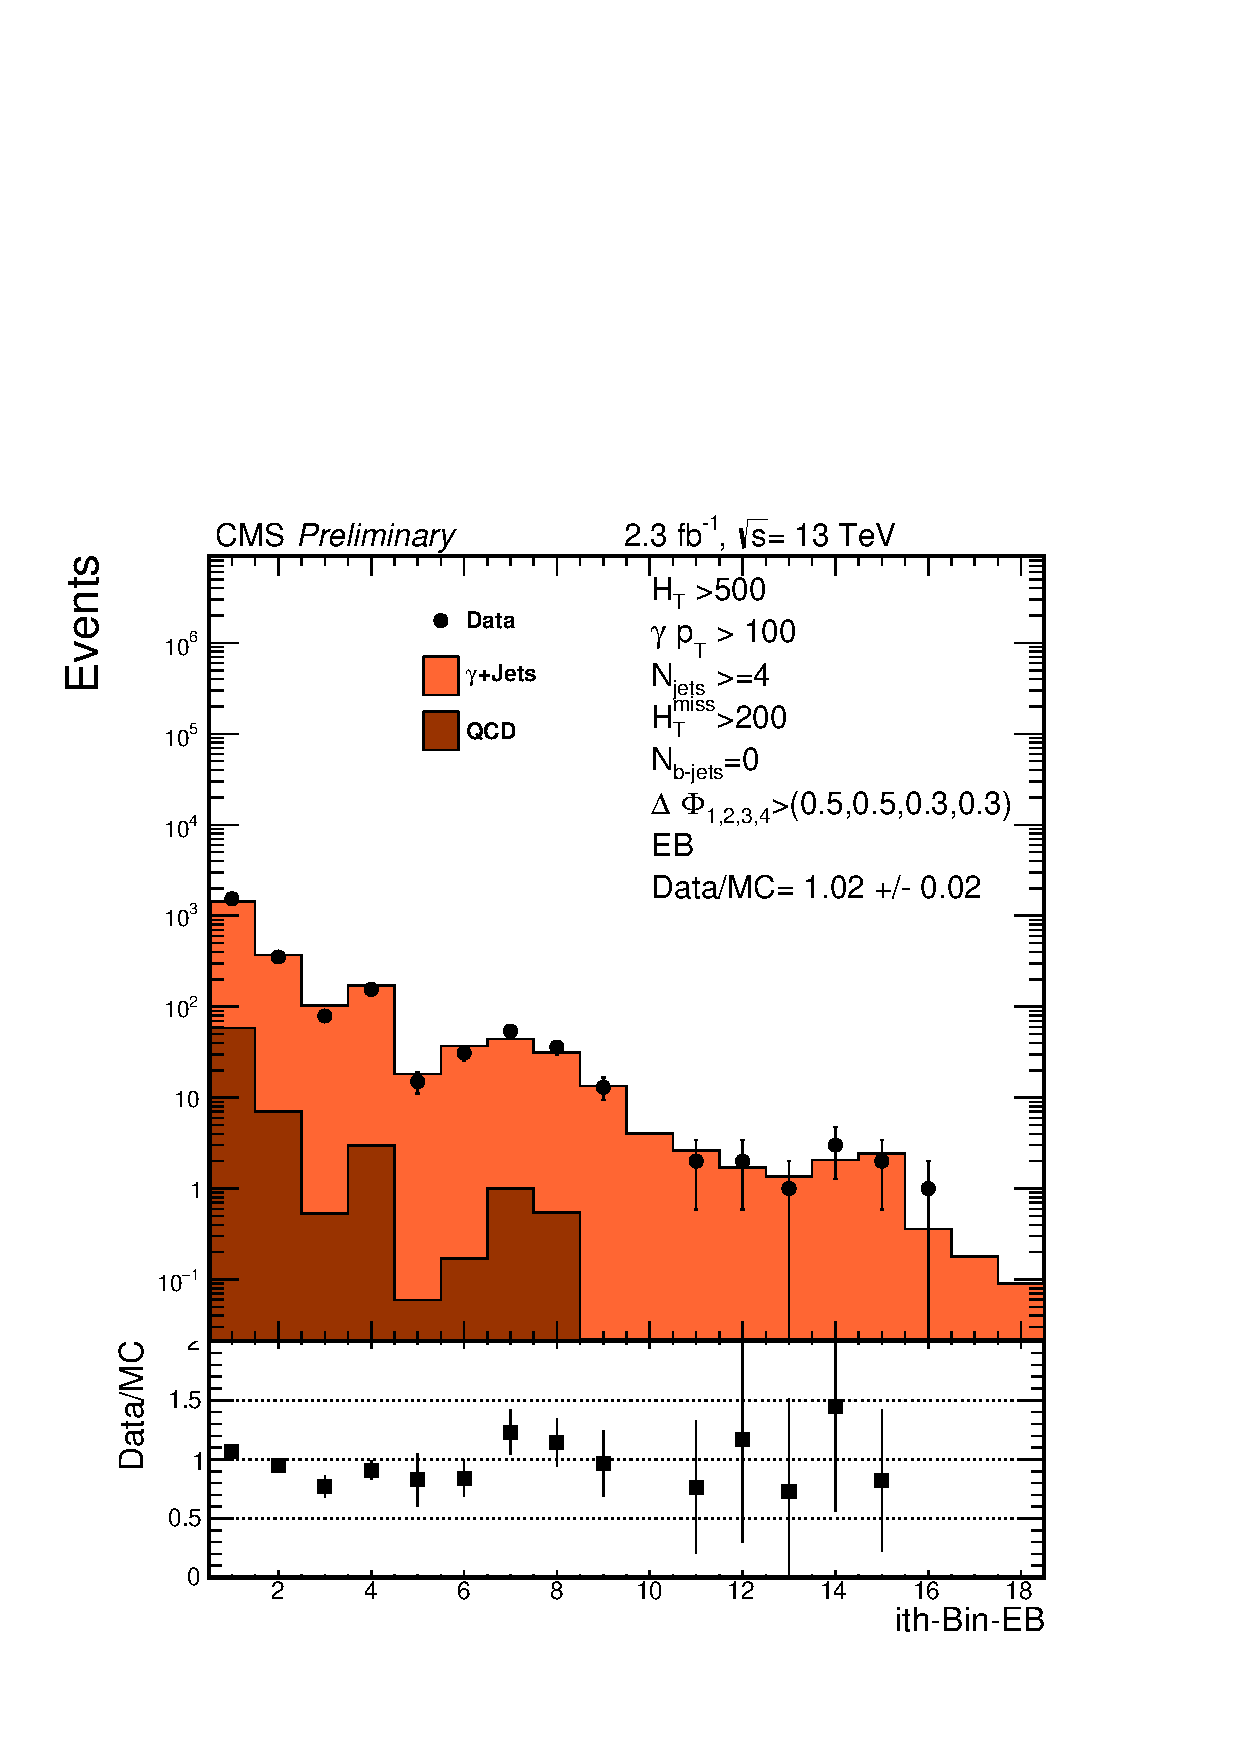
\includegraphics[width=0.30\textwidth]{/home/bibhu/Desktop/PhDThesis/PhDThesis/synopsis/ith-Bin-EB__Data_MC_EB.pdf} % ADDNEWPLOT 
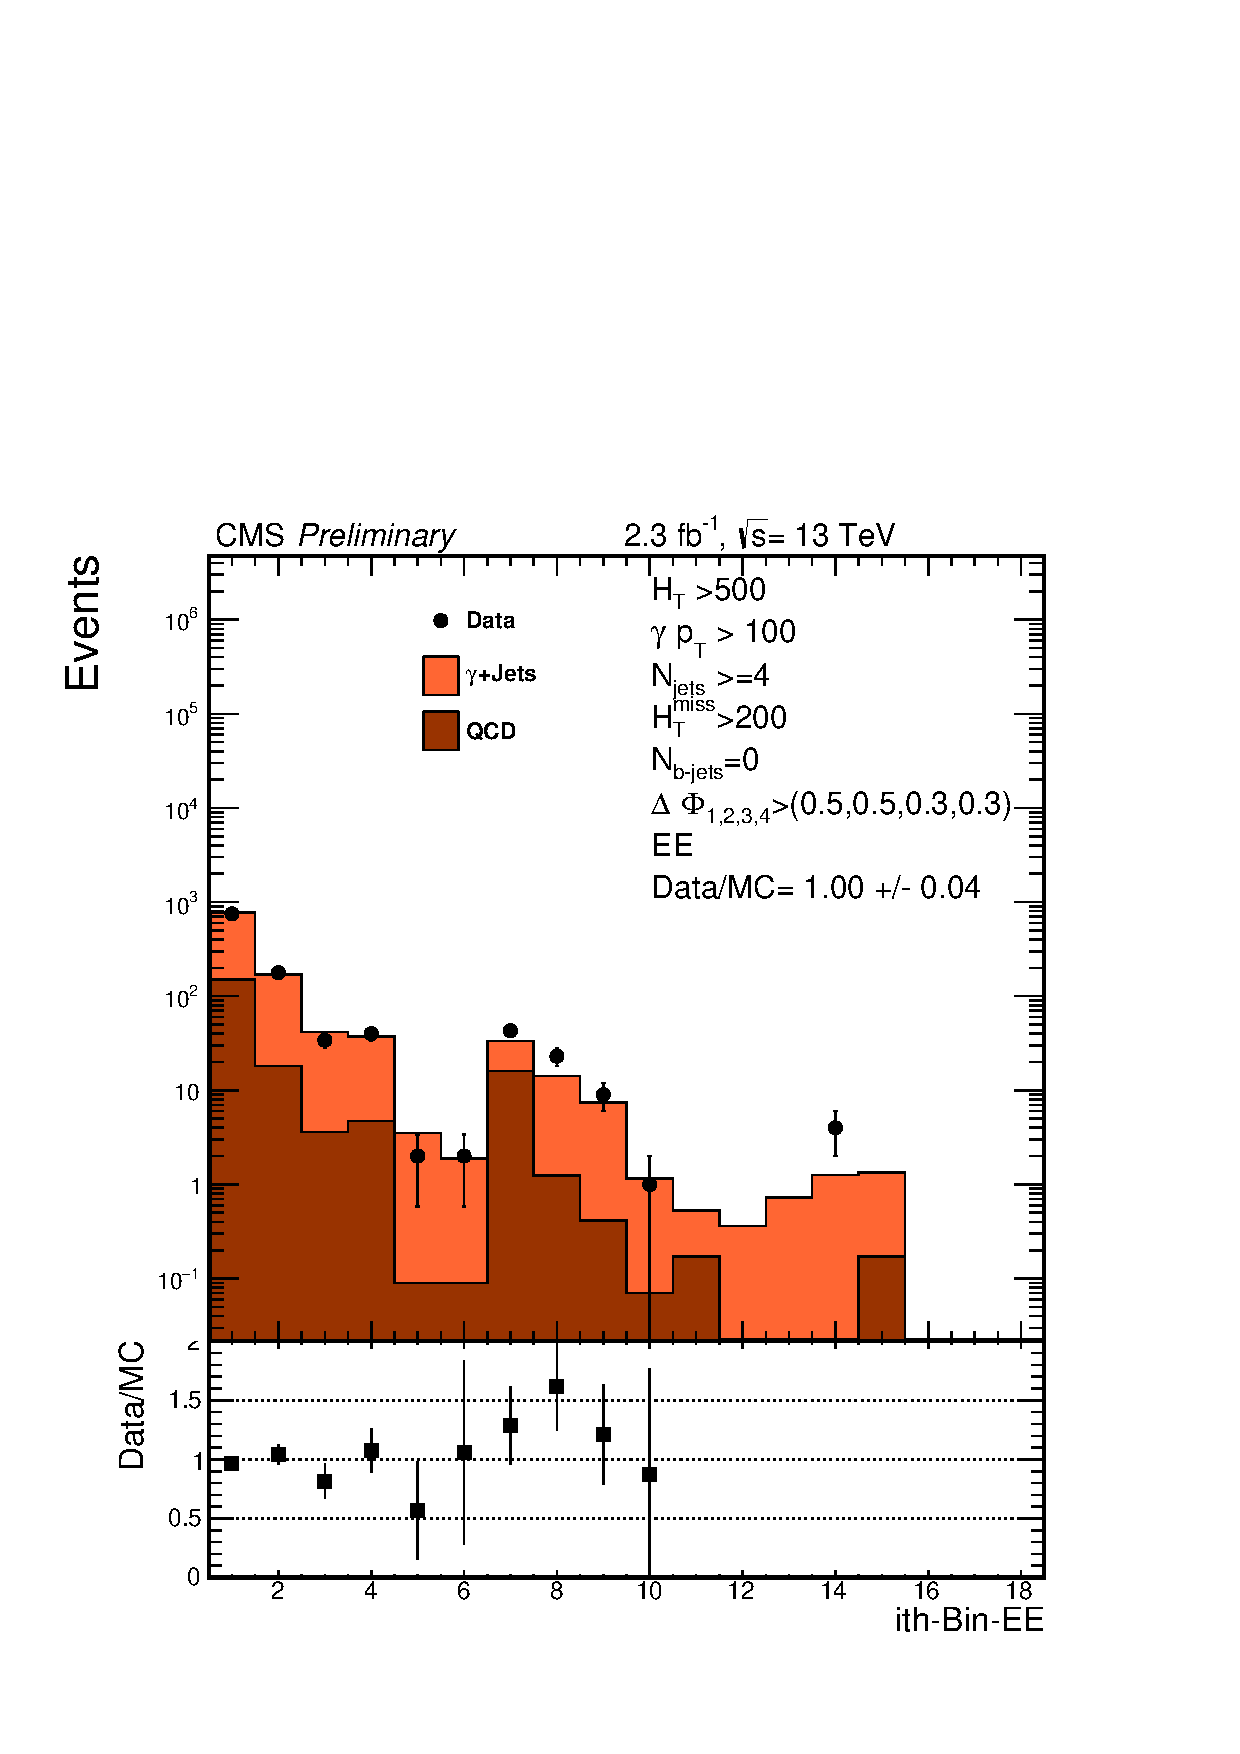
\includegraphics[width=0.30\textwidth]{/home/bibhu/Desktop/PhDThesis/PhDThesis/synopsis/ith-Bin-EE__Data_MC_EE.pdf} % ADDNEWPLOT 
\caption{Physics ratio $\rm R_{Z(\nu\bar{\nu})/\gamma}$ (left), numbers of observed events in the photon control samples in barrel(EB, middle) and endcap(EE, right) compared to simulation.}
\label{fig:GJdatavsmc}
\end{center}
\end{figure}
$DR$, called the double ratio, is a correction factor to the physics ratio $R_{Z(\nu\bar{\nu})/\gamma}$. This is calculated by measuring the $R_{Z(\ell^{+}{\ell^{-}})/\gamma}$ both in data and simulation and then taking the ratio.

Prompt photons can be distinguished from non-prompt photons by the shapes of their 
showers in the ECAL, as described by the well-known quantity $\sigma_{i\eta i\eta}$.  
The purity is determined with a two-component fit to the $\sigma_{i\eta i\eta}$ distribution 
in the photon control sample.  The PDF for the prompt component is fitted directly in data
using a gaussian function.

Fig ~\ref{fig:GJdatavsmc} shows the data vs MC simulation for 18 kinematic bins (0-btag) where a  photon$+$ jet method is employed. 
\paragraph{\underline{Lost lepton}: }
SM events (mostly $\rm t\bar{t}$ and W+jets) with muons or electrons
can satisfy the event selection and enter the signal sample as lost-lepton background
if the requirements for any of the following analysis steps are not satisfied

\begin{itemize}
\item Kinematic acceptance,
\item Reconstruction, or
\item Isolation.
\end{itemize}
The basic idea behind our data-driven method to evaluate
the lost-lepton background is to select
single-lepton control samples (CS) in the data,
through inversion of the lepton vetoes,
and to weight each CS event
by a factor that represents the probability for a lost-lepton event
to appear with
the corresponding search-variable values: $\rm H_{T}$, $\rm H_{T}^{miss}$, $\rm N_{jet}$, and $\rm N_{jet}^{miss}$.
The weights are determined through evaluation of the efficiencies
for each analysis step.
The weighted distributions of the search variables,
summed over the events in the CS,
define the predicted lost-lepton background in the respective search regions.
\paragraph{\underline{QCD}: }
The $\rm H_{T}^{miss}$ in QCD multijet events is almost always due to a mismeasured jet in the event,
       thus the $\rm H_{T}^{miss}$ direction is usually close to the jet.
       The $\rm \Delta \phi$ variable is the minimum $\phi$ difference between $\rm H_{T}^{miss}$ and one of the four
       highest $\rm p_{T}$ jets.


       The low $\rm \Delta \phi$ region is significantly enriched in QCD events.
       The sample of events with the $\rm \Delta \phi$ requirement inverted
       (i.e., $\Delta \phi_1<0.5$ or $\Delta \phi_2<0.5$ or $\Delta \phi_3<0.3$ or $\Delta \phi_4<0.3$)
       serves as the QCD control sample.
       %Figure~\ref{fig:qcd-mdp-split1d} shows \dphi distributions for zero-lepton events
       %passing the baseline selection in bins of \HT, \MHT, and \njets.
       The background at high $\rm \Delta \phi$, is estimated from the QCD yield at low
       $\rm \Delta \phi$ and a high/low ratio $R^{\rm QCD}$ for the QCD component.
       The $\rm \Delta \phi$ distribution  shows that the high/low ratio
       has some dependence on the search variables $\rm H_{T}$, $\rm H_{T}^{miss}$, and $\rm N_{jet}$.
       We model this dependence by assuming that it factorizes.  That is, we assume the $\rm H_{T}$
       dependence does not depend on $\rm H_{T}^{miss}$ or $\rm N_{jet}$ and similarly for $\rm H_{T}^{miss}$ and $\rm N_{jet}$.
\paragraph{\underline{Hadronic tau}: }

To evaluate the $\rm t\bar{t}$, single-top and W+jets backgrounds
that arises when a W boson decays to a neutrino and
a hadronically decaying $\tau$ lepton ($\tau^{h}$),
we employ a tau-template method. %~\cite{RA28TeVpaper,RA28TeVan,RA2-2011pub,RA2-2010pub}.
In this approach, the $\tau^{h}$ background is estimated from a control sample (CS)
of $\mu$+jets events,
which we select by requiring exactly one muon with $\rm p_{T}>20$ GeV and $|\eta|<2.1$. 
This single-muon CS is
mainly composed of $\rm t\bar{t}(\rightarrow \mu\nu)$ and W($\rightarrow \mu\nu$)+jets events.
Since both $\mu$+jets and $\tau^{h}$+jets events 
arise from the same underlying process,
the hadronic components of the two event classes are expected to be the same,
aside from the response of the 
detector to a muon or a $\tau^{h}$ jet. 
The basic idea behind the method
is to smear the muon $\rm p_{T}$ in the CS events,
using MC-derived response functions (the ``templates''),
in order to emulate the $\tau^{h}$ jet response.
Global hadronic variables such as $\rm N_{jet}$, $\rm H_{T}$, and $\rm H_{T}^{miss}$
are then recomputed, and the full analysis procedure is subsequently applied. 




%/////////////////////////////////


\subsubsection{Uncertainties}

Various kinds of systematic and statistical uncertainties that are considered in the analysis. The uncertainties that result from the background estimations including data control region statistics, purity of control region , CR trigger efficiency etc. are discussed in details in Ref. ~\cite{CMS-PAS-SUS-15-002}. Below we briefly describe various systematic uncertainties that affect the expected signal yield.


\begin{itemize}

\item {\bf Luminosity:} A flat 4.6 $\%$ uncertainty on luminosity is propagated to the signal yield. 

\item {\bf b-tag efficiency:} The b-tagging and mistagging scale factors are functions of the jet
 $\rm p_{T}$ and $\eta$. The scale factors are varied by their uncertainties and these variations are propagated as migrations between the different signal bins.

\item {\bf MC statistics:} The MC statistical uncertainties are propagated to the signal yield 

\item {\bf Trigger efficiency:}The trigger efficiencies are measured in the data.
The effect of the statistical and systematic uncertainties is at most 1.1 $\%$ at low $\rm H_{T}^{miss}$.

\item {\bf Pileup reweighting: }The uncertainties in the pileup reweighting correction are derived from the uncertainties in the minimum bias cross section and the difference between the expected and  observed number of interactions in the data. The minimum bias cross section in the 13 TeV is estimated to be 69 mb with an uncertainty of $\pm$5$ \%$. The correction is varied according to these uncertainties, with a maximum effect of 0.5 $\%$.

\item {\bf Scale:} The uncertainty is calculated from using the envelope of weights from varying the renormalization and factorization scales. The effect on the yield of non-compressed samples is less than 0.1 $\%$ and on compressed samples ranges from 1 $ \%$ to 3 $ \%$.

\item {\bf ISR: } The effect on the yield of non-compressed samples is less than 0.1 $\%$ and on compressed samples ranges from 3 $\%$ to 11 $\%$.


\item {\bf Jet Energy Corrections: } The jet energy corrections (JECs) are varied using the $\rm p_{T}$
and $\eta$ dependent jet energy scale uncertainties from the official database, with a separate set of corrections for the fast simulation samples. The overall effect ranges from 0.5 $\%$ to 4$\%$. 

\item {\bf PDF: } The LHC4PDF prescription for the uncertainty on the total cross section is included as $\pm$1 $\sigma$ bands in the results. 

\end{itemize}
 



%///////////////////////////////////////


\subsubsection{Results}
The data in the signal regions are found to be in 
generally good agreement with the predicted backgrounds. Therefore we do not see any evidence for new physics. For the 72
search bins, the observed data and the pre-fit predictions for each background component are shown in Fig.~\ref{fig:Datavsbkg}. The 95\% confidence-level   (CL) upper limit is calculated on the production cross section taking all 72 bins. The upper limits on the signal cross section and the exclusion curves are shown in Fig.~\ref{fig:Limit2015Synop}. For calculating the upper limits we use  a test  statistic  $\rm q_{\mu}$ = $-$2ln($L_{\mu}/L_{max}$), where $L_{max}$ is the maximum likelihood determined by allowing all parameters including the SUSY signal strength $\mu$ to vary and $L_{\mu}$ is the maximum likelihood for a fixed signal strength . The details of the statistical procedure can be found in Ref.~\cite{CMS-NOTE-2011-005}.  For an explanation of the treatment of uncertainties, we refer to Ref. ~\cite{CMS-PAS-SUS-15-002}. As can be seen from the plots in Fig.~\ref{fig:Limit2015Synop} the observed exclusion limits for low LSP masses lie around 1600 GeV both for four top and four b-quark final state, for four light quark final state, it is around 1450 GeV of gluino mass. The small disagreement of observed exclusion curves with the expected ones can be ascribed to the small insignificant excesses of events we see in various bins.  
\begin{figure}[h]
\begin{center}
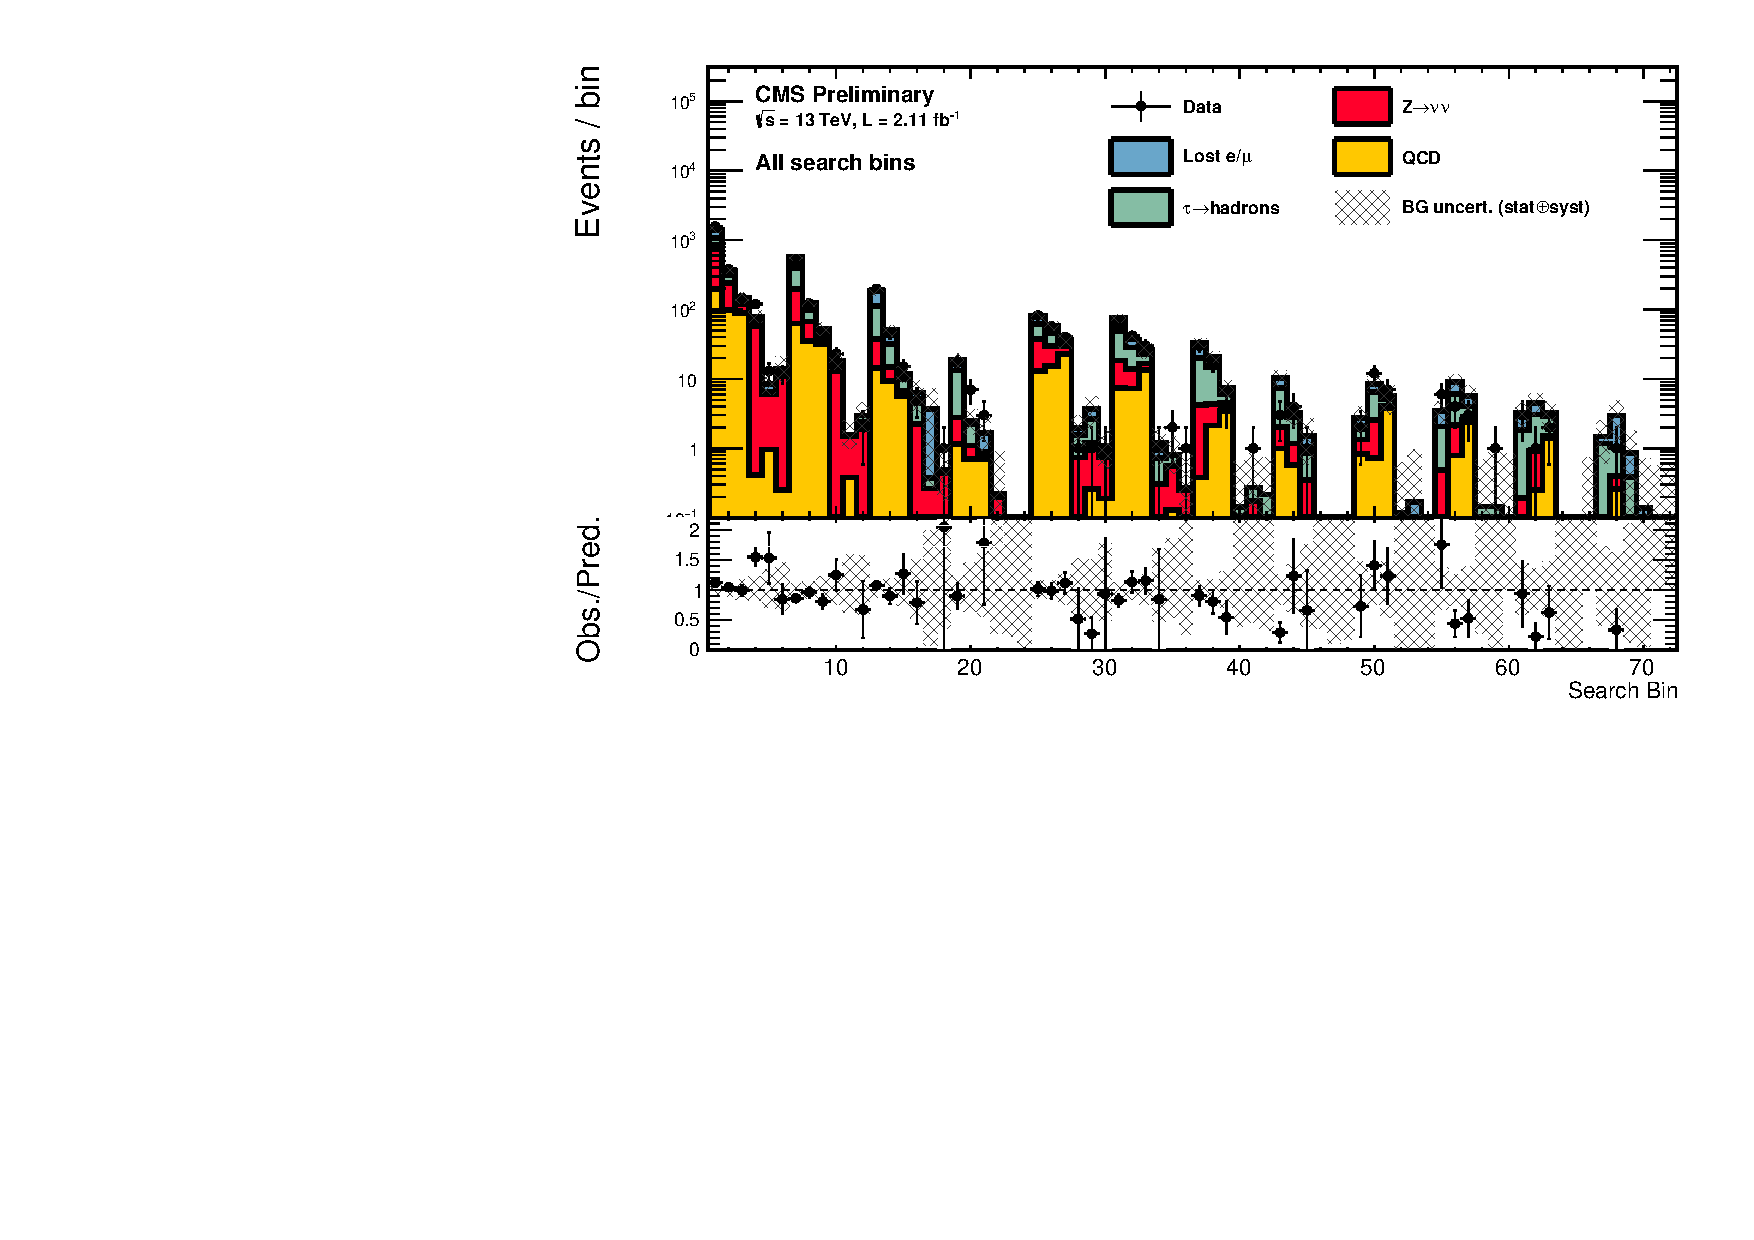
\includegraphics[width=0.70\textwidth]{/home/bibhu/Desktop/PhDThesis/PhDThesis/synopsis/prefit-results-all-log.pdf}
\caption{\label{fig:Datavsbkg} Data vs. the SM background before fit}
\end{center}
\end{figure}
\begin{figure}[h]
\centering
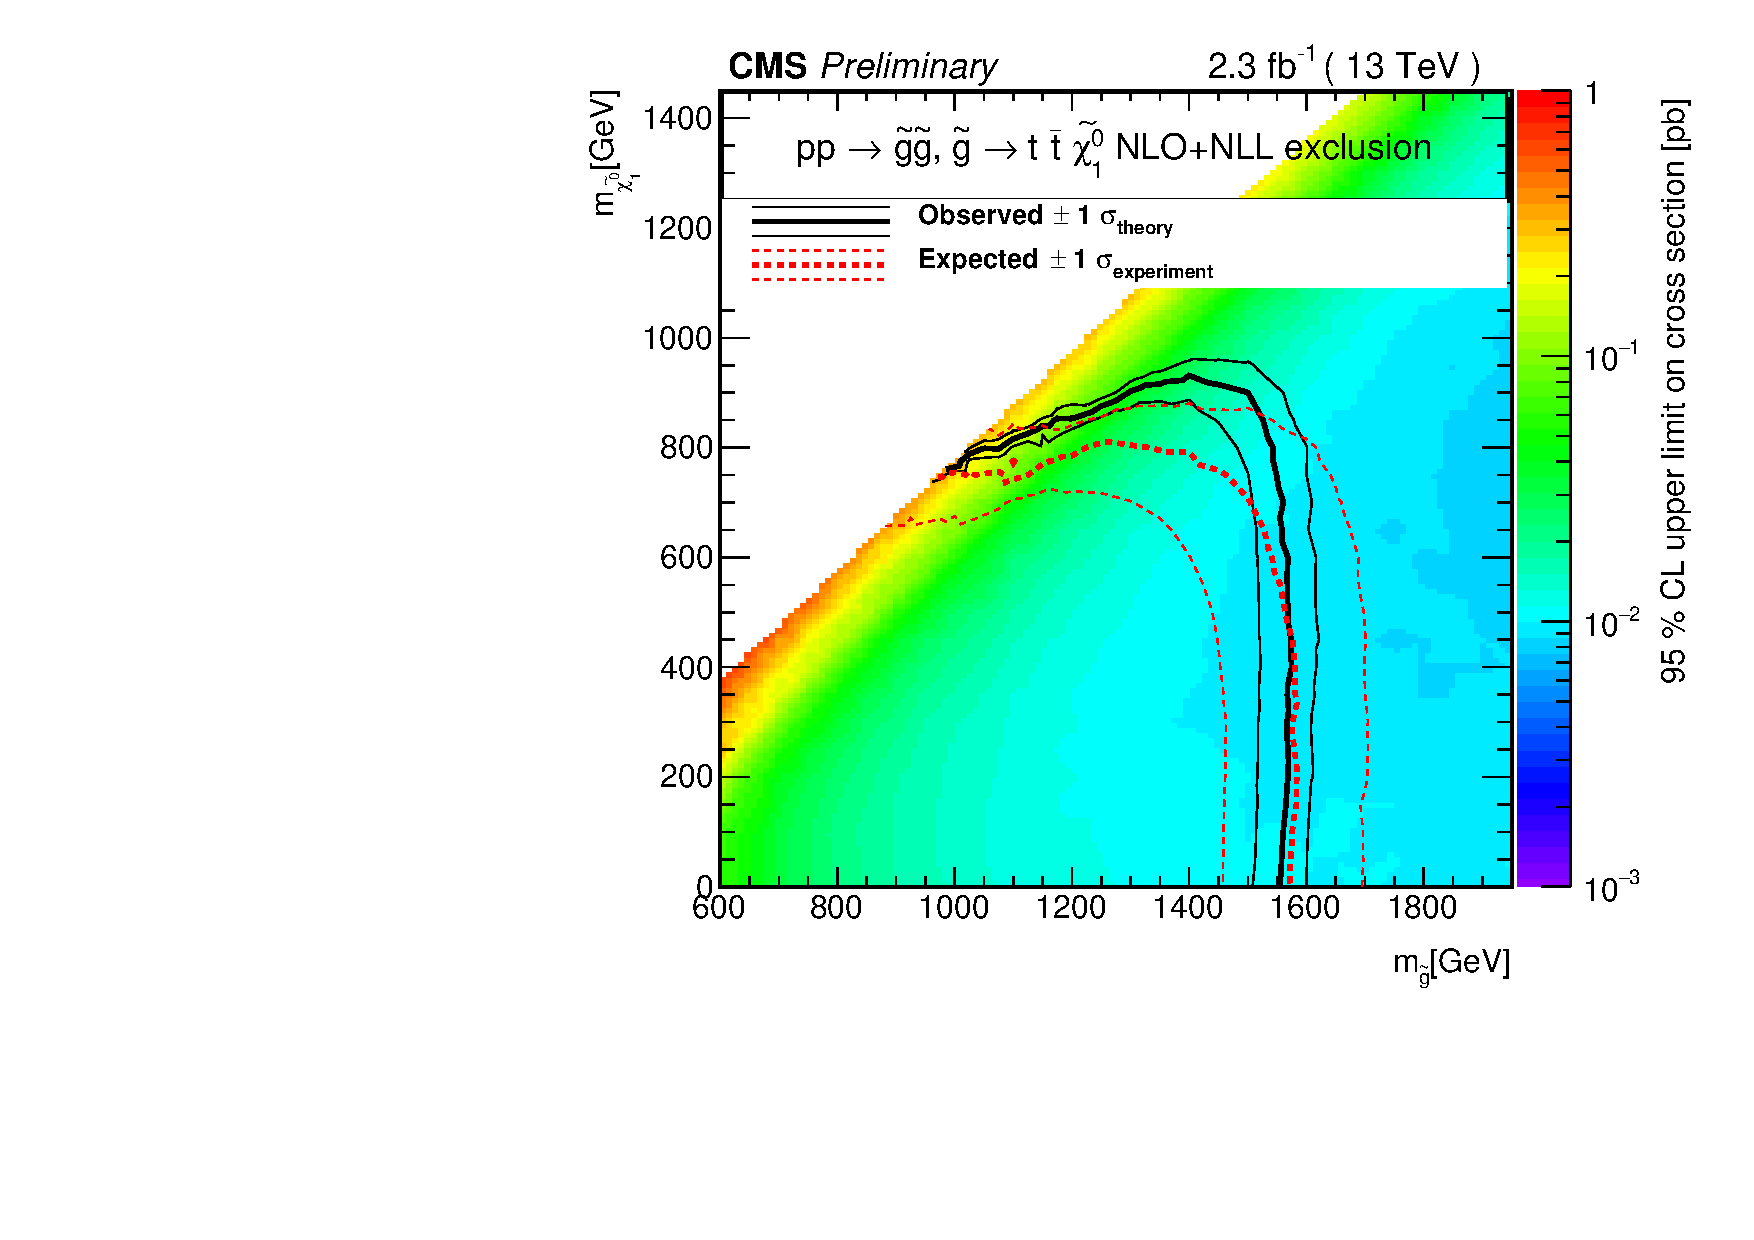
\includegraphics[width=0.32\textwidth]{/home/bibhu/Desktop/PhDThesis/PhDThesis/synopsis/T1tttt_2p3_limit.pdf}
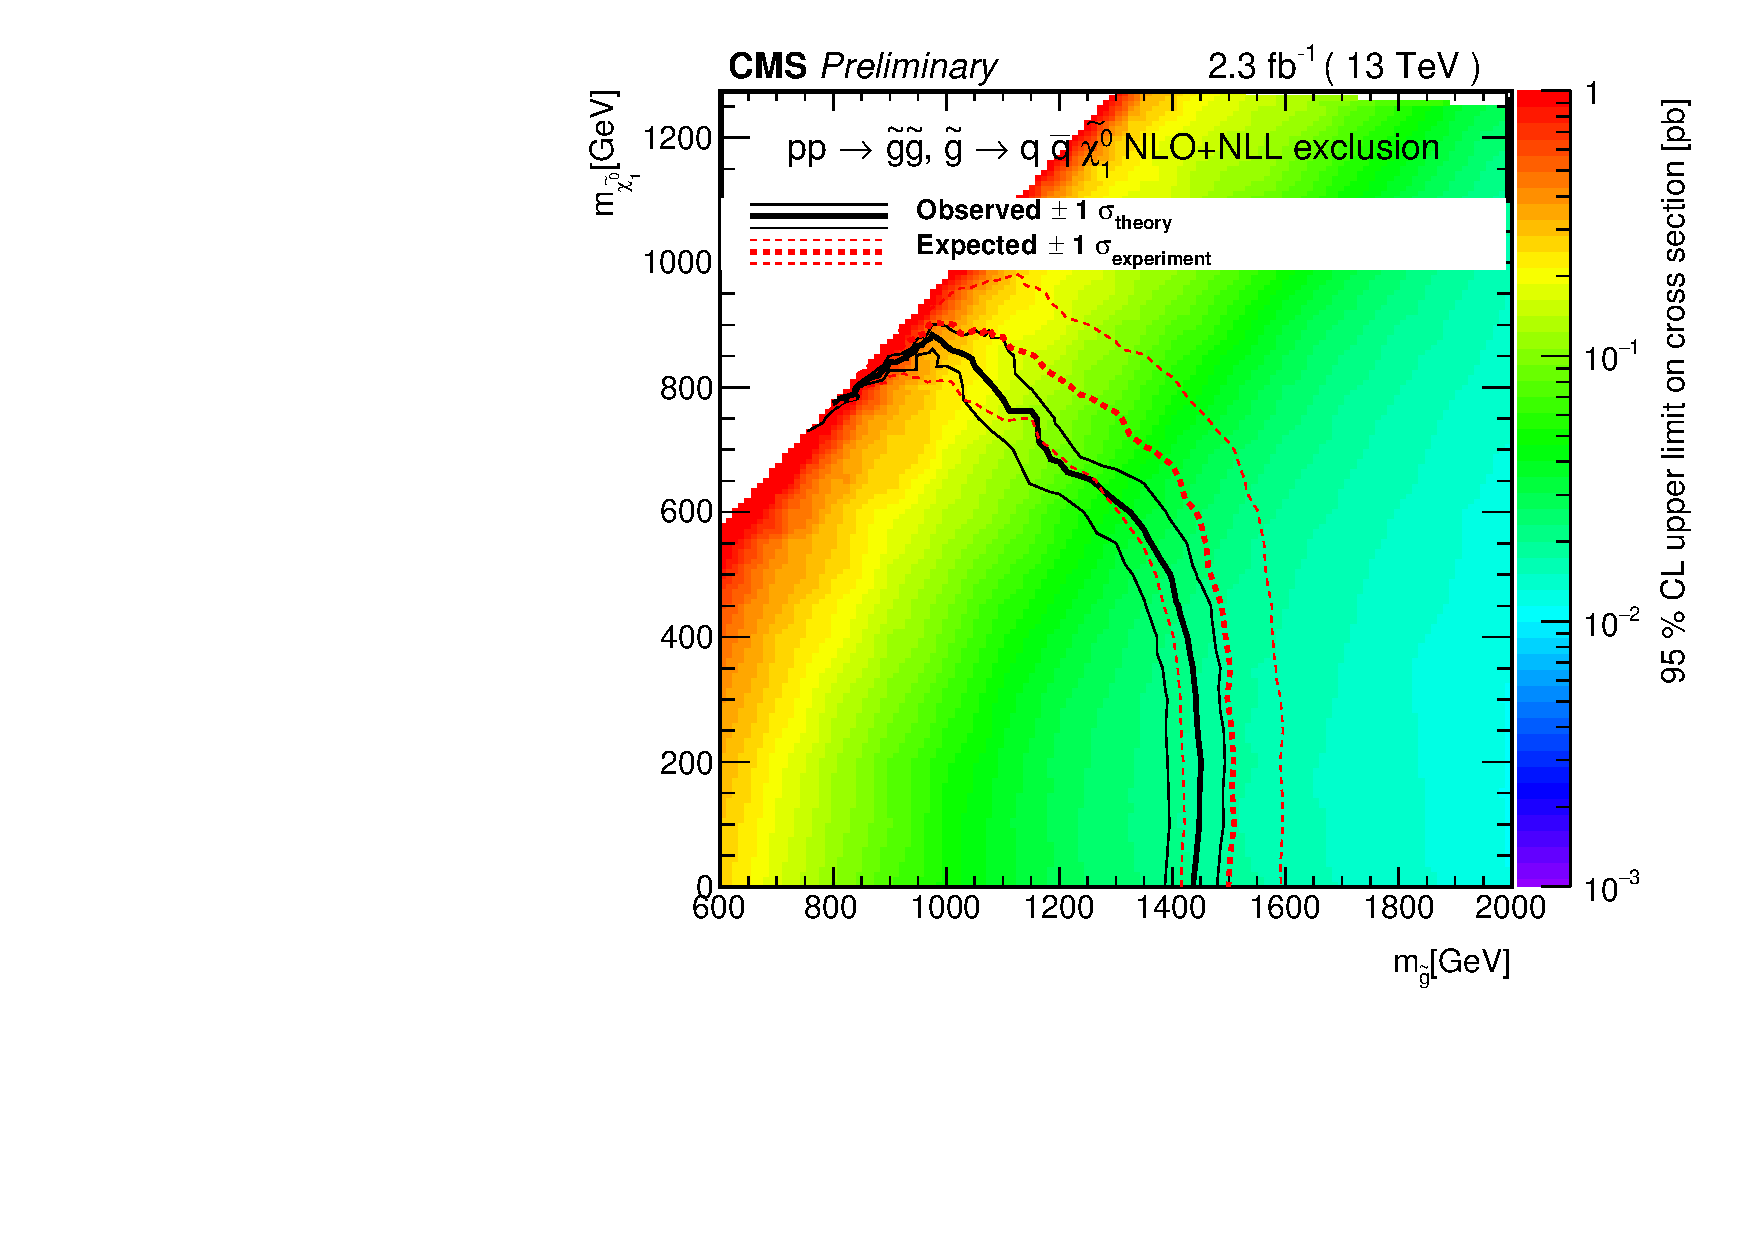
\includegraphics[width=0.32\textwidth]{/home/bibhu/Desktop/PhDThesis/PhDThesis/synopsis/T1qqqq_2p3_limit.pdf}
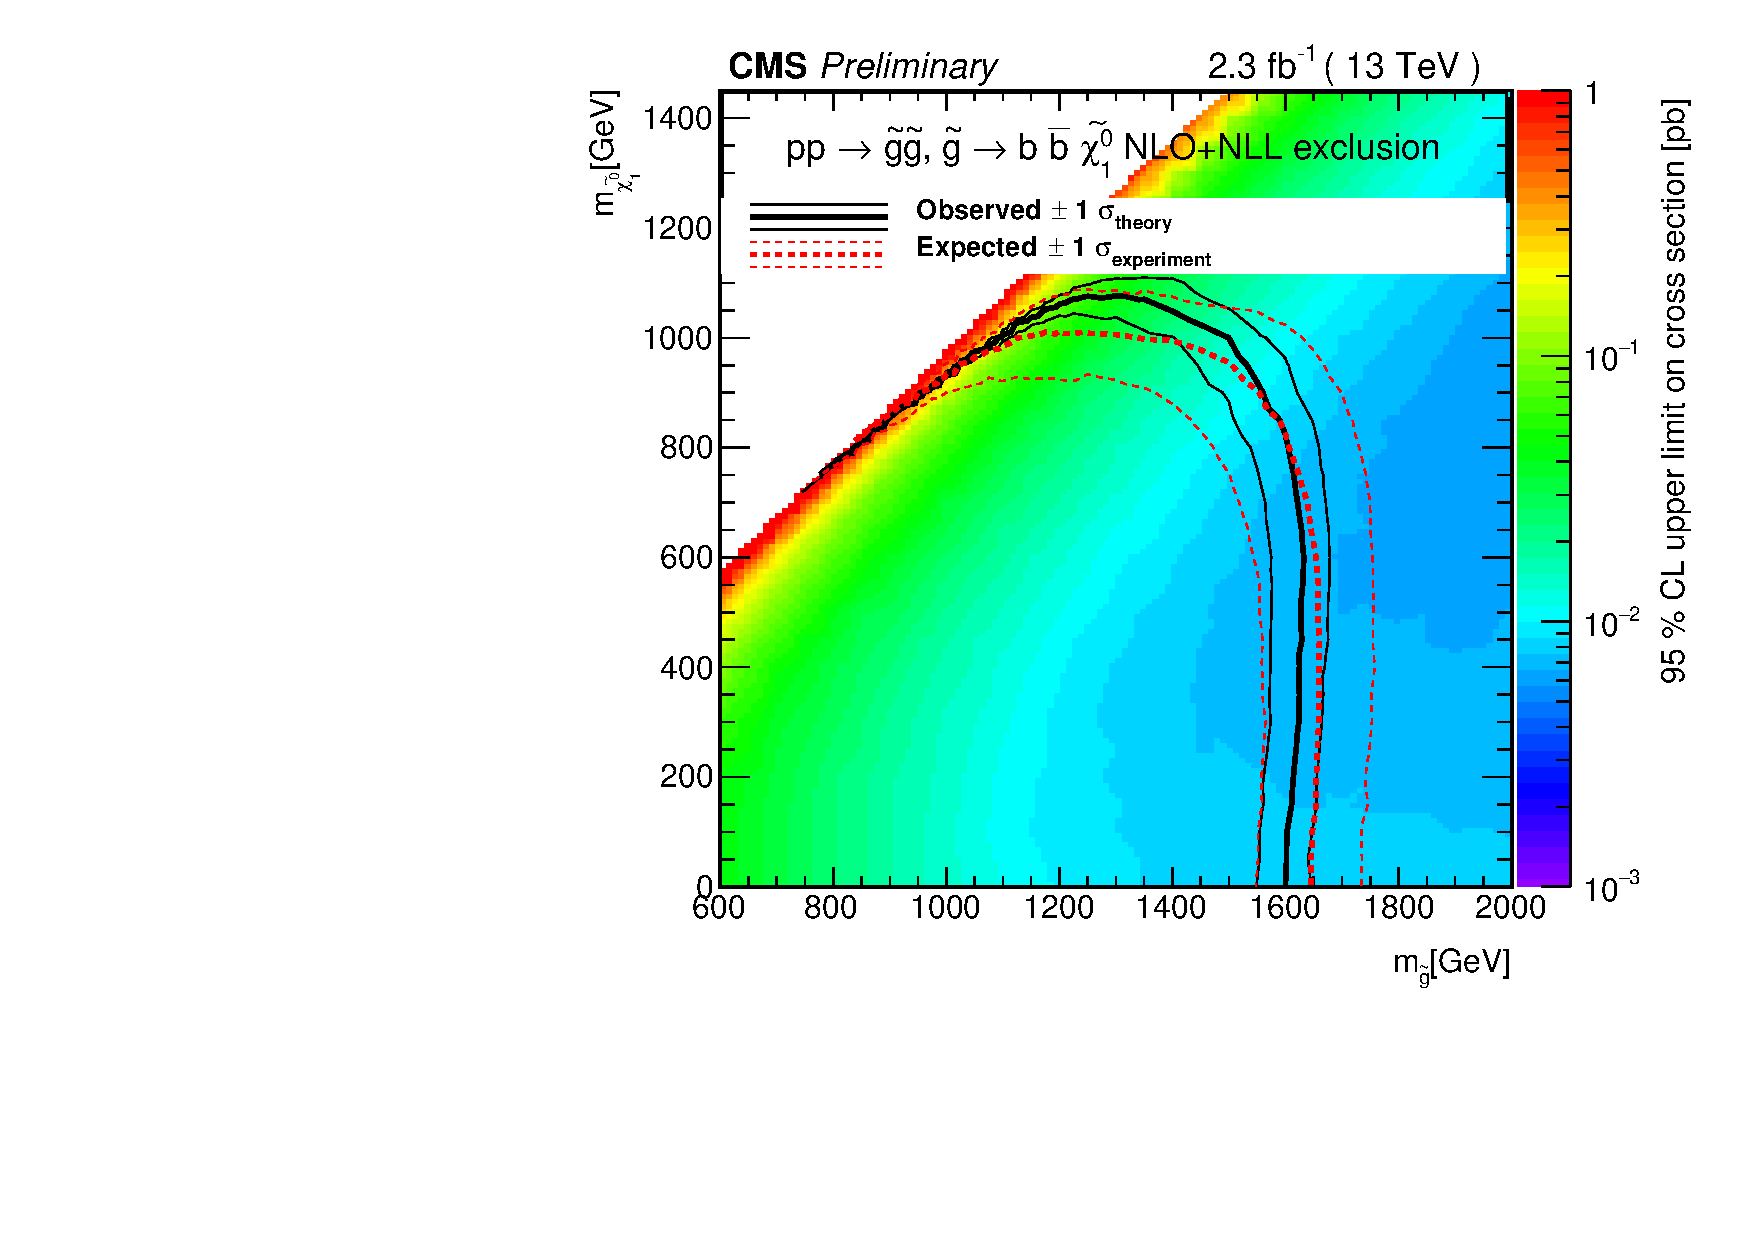
\includegraphics[width=0.32\textwidth]{/home/bibhu/Desktop/PhDThesis/PhDThesis/synopsis/T1bbbb_2p3_limit.pdf}
\caption{\label{fig:Limit2015Synop}The 95\% CL upper limits on the production cross sections for four top quark(left),four light quark(middle) and four b-quark(right) in the final state. }
\end{figure}

\newpage
\subsection{Study on 12.9 $\rm fb^{-1}$ of 2016 Data}
In 2016 we lowered the $\rm H_{T}$ and $\rm N_{jet}$ thresholds to enhance the search sensitivity to some stop and squark production models. Also the number of bins is changed from 72 to 160 for an increased sensitivity. The important event selection and search region definitions that are different with respect to the 2015 analysis are described below. 
\subsubsection{Search Region and Event Selection}

The following requirements define the selection criteria for signal event candidates:
\begin{itemize}
\item $\rm N_{jet}$ $\geq$ 3, where the jets must satisfy $|\eta|$ $<$ 2.4; we change the jet multiplicity threshold to 3 because of our change in focus to direct squark-pair production in addition to gluino-pair production;
\item $\rm H_{T}$  $>$ 300 GeV;
\item $\rm H_{T}^{miss}$ $>$  300 GeV ;
All other criteria remain almost the same as for the 2015 analysis (see Sec. 4.1.1).

\end{itemize}
The search is performed in the following 160 ($=4\times4\times10$) exclusive intervals of the four search variables:
\begin{itemize}

 \item ${\bf 3 }$ $\rm N_{jet}$ bins: 3-4, 5-6,7-8, $\geq$9;
 \item ${\bf 4 }$ $\rm N_{b-jet}$ bins: 0, 1, 2, $\geq$3;
 \item  ${\bf 10 }$ bins in $\rm H_{T}$ and $\rm H_{T}^{miss}$: defined below



\begin{center}
\begin{tabular}{ c c c }
 Bin & $\rm H_{T}$ range [GeV] & $\rm H_{T}^{miss}$ range [GeV] \\ 
  1: & 300$-$500 & 300$-$350 \\ 

  2: & 500$-$1000 & 300$-$350 \\  

  3: & $>$1000 & 300$-$350\\

  4:&  350$-$500 & 350$-$500\\

  5: & 500$-$1000 & 350$-$500\\

  6: & $>$1000 & 350$-$500\\

  7: & 500$-$1000 & 500$-$750\\

  8: & $>$1000 & 500$-$750\\

  9: & 750$-$1500 & $>$750\\

 10: & $>$1500 & $>$750\\


\end{tabular}
\end{center}


 
\end{itemize}


\subsubsection{Background Estimation}
Similar methods to estimate various SM backgrounds are employed in this analysis even though their relative composition has changed from 2015 owing to the change of baselines. As the phase space has changed, these methods are optimized accordingly. Below we describe the changes for the Z($\rightarrow \nu \bar{\nu}$)+jets background. Details of other background estimations can be found in Ref.~\cite{CMS-PAS-SUS-16-014}.

\underline{Z($\rightarrow \nu \bar{\nu}$)+jets: } 

\begin{itemize}

\item A new high-statistics MC sample is used to calculate the transfer factor $\rm R_{Z/\gamma}$ helping to  reduce the related systematic uncertainty.

\item For the calculation of photon purity, a charged isolation template is used instead of $\sigma_{i\eta i\eta}$ as we find it to have a better performance.

\item Trigger for the photon control region is also changed. 

Note that due to the change in $\rm H_{T}^{miss}$ and $\rm N_{jet}$ threshold the contribution of Z background is increased in many bins.

\end{itemize}

\subsubsection{Uncertainties}

The uncertainties are treated in the same way as it is done with 2015 data. The $\%$ uncertainties are also similar to the previous analysis.




\subsubsection{Results}
Fig.~\ref{fig:Datavsbkg2016} shows the predicted background vs. the observed data. The background is found to be statistically compatible with data for all 160 regions. Thus, we do not see any evidence for new physics. The  95\% CL upper limits on the cross section are shown in Fig.~\ref{fig:Limit2016Synop}. These plots show significant improvements in terms of expected limits when compared to the previous results with 2.3 $\rm fb^{-1}$ of data (Fig.~\ref{fig:Limit2015}). The mismatch between the observed and expected curves owing to the deficit of events in some of the bins.   
\begin{figure}
\centering
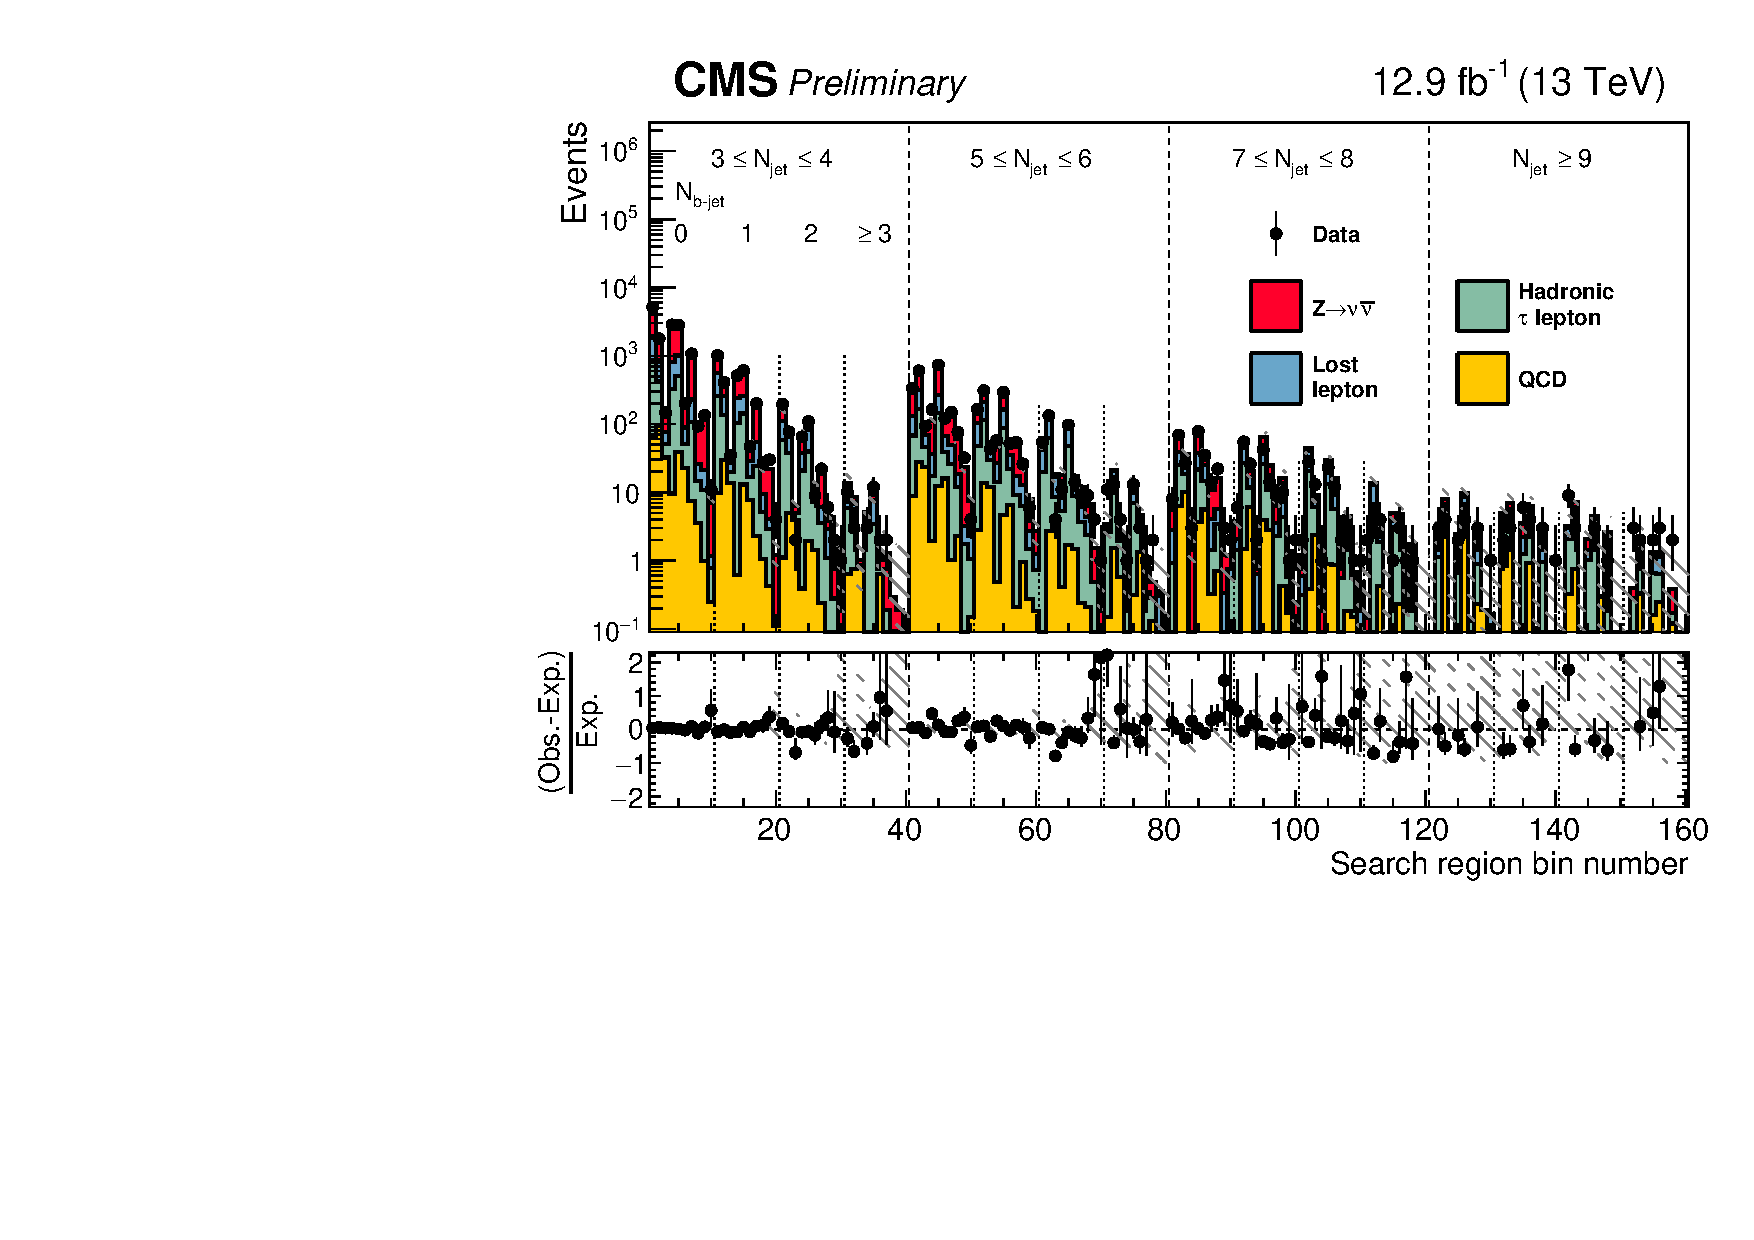
\includegraphics[width=10cm,height=5cm]{/home/bibhu/Desktop/PhDThesis/PhDThesis/synopsis/results-plot-prefit-12_9-log.pdf}
\caption{\label{fig:Datavsbkg2016} Data vs. the SM background before fit.}
\end{figure}
\begin{figure}[h]
\centering
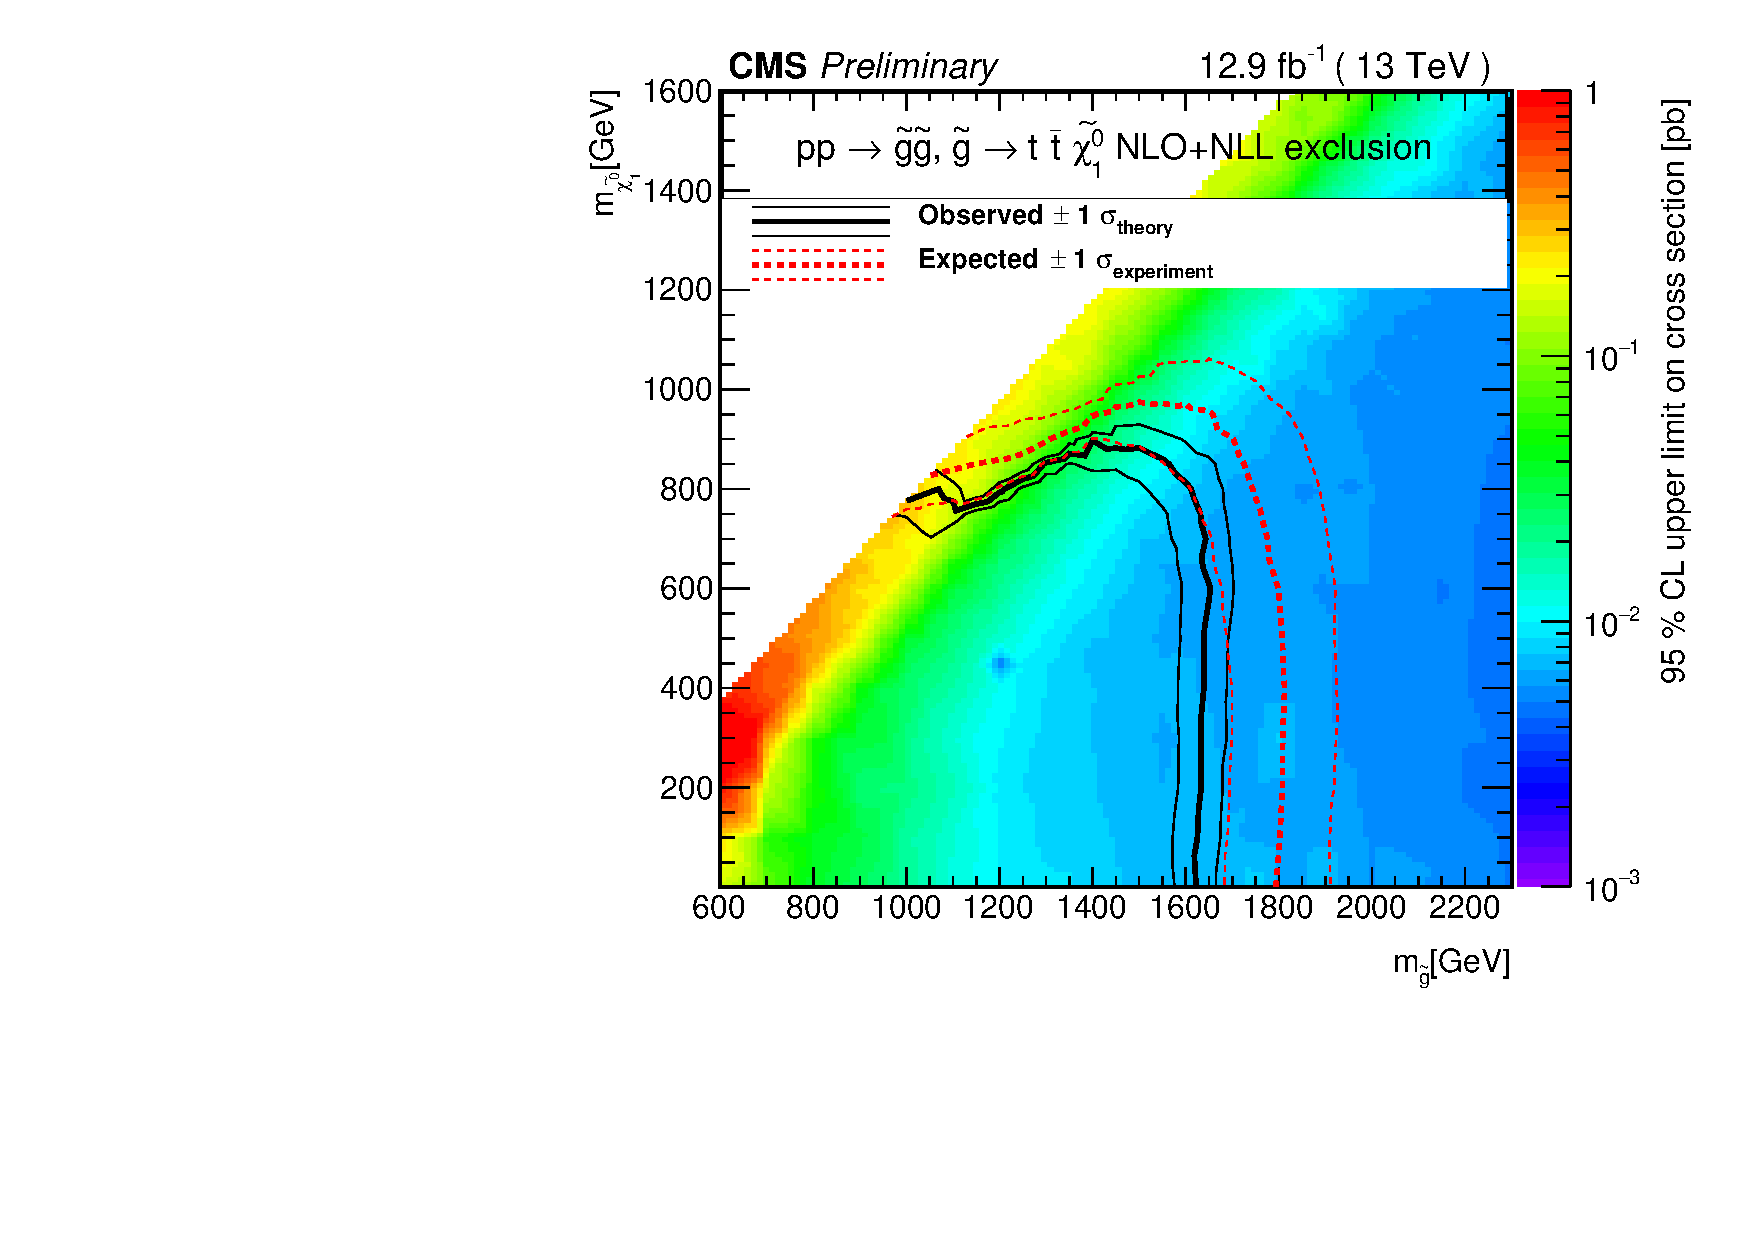
\includegraphics[width=0.32\textwidth]{/home/bibhu/Desktop/PhDThesis/PhDThesis/synopsis/T1tttt_12p9_limit.pdf}
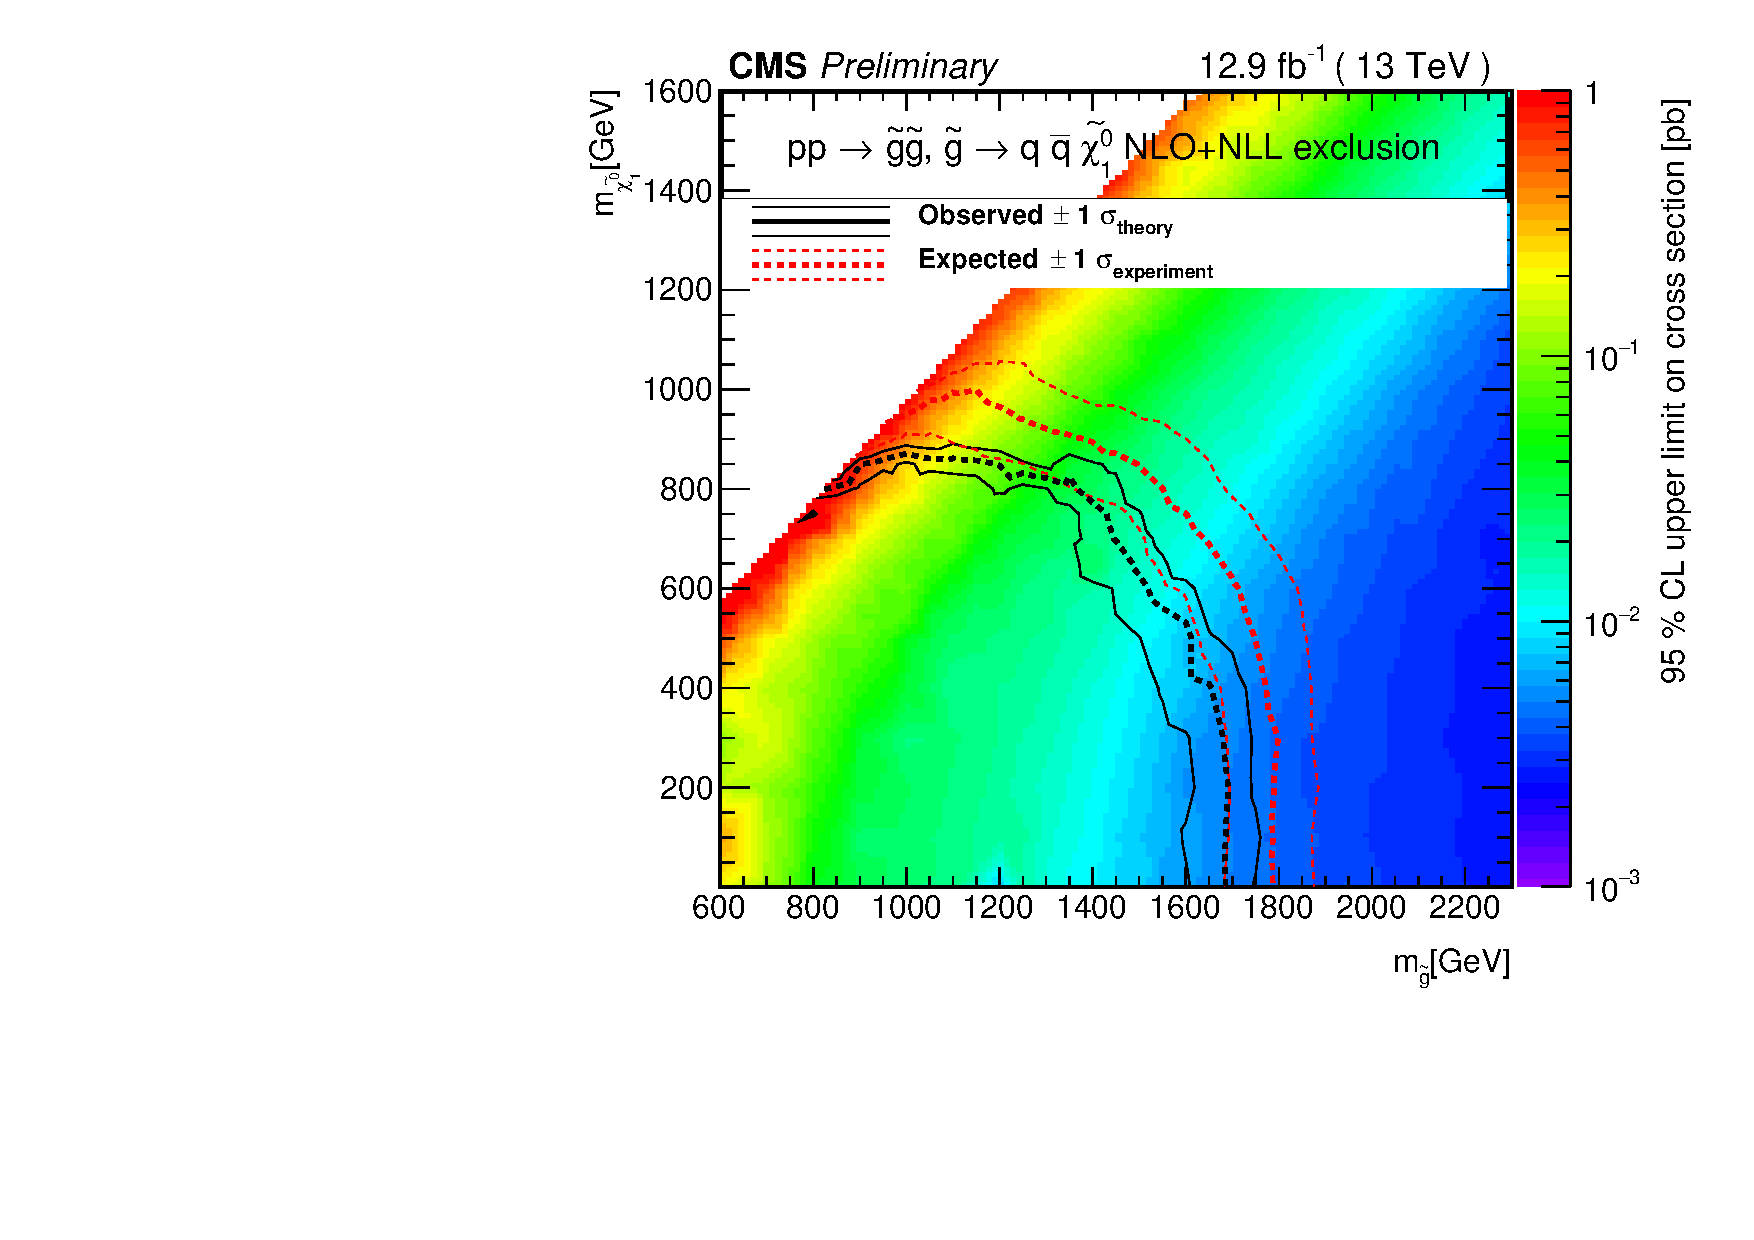
\includegraphics[width=0.32\textwidth]{/home/bibhu/Desktop/PhDThesis/PhDThesis/synopsis/T1qqqq_12p9_limit.pdf}
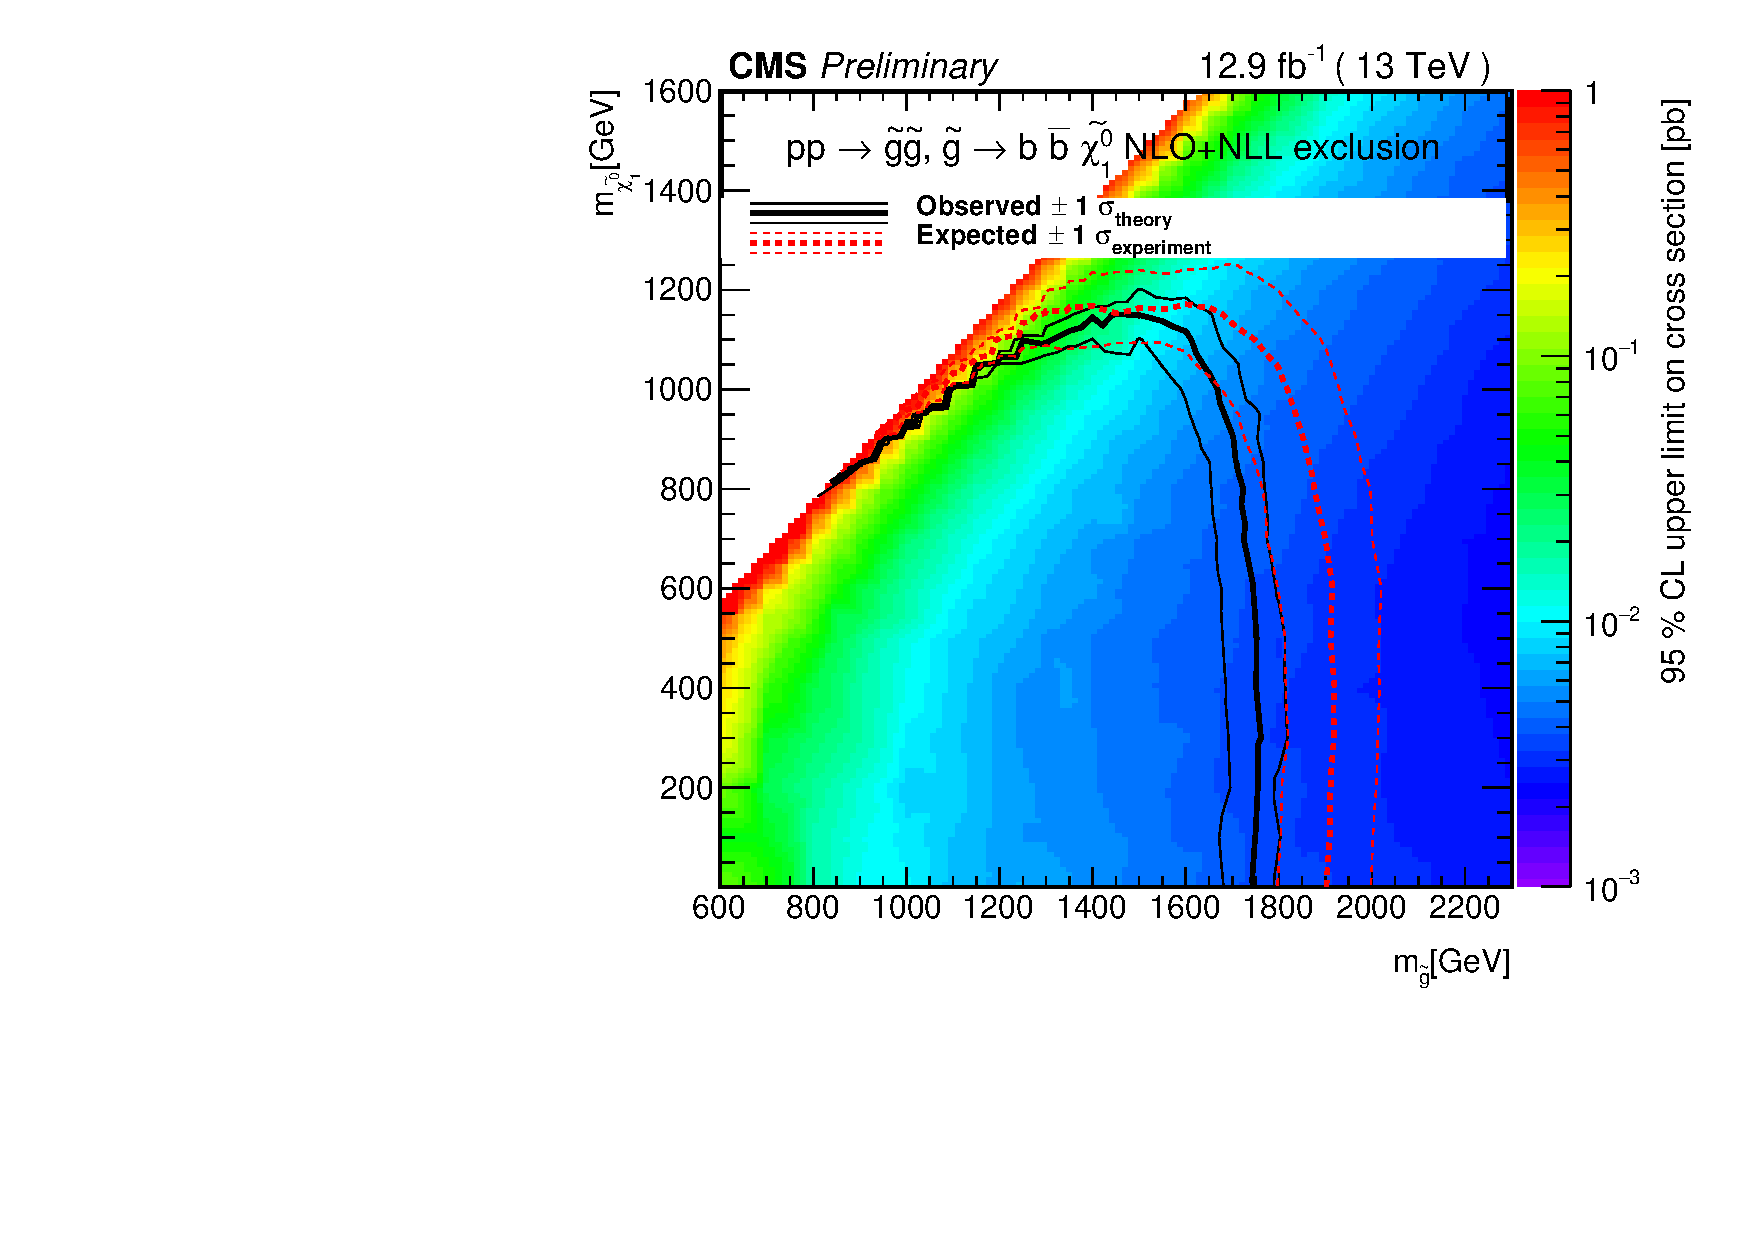
\includegraphics[width=0.32\textwidth]{/home/bibhu/Desktop/PhDThesis/PhDThesis/synopsis/T1bbbb_12p9_limit.pdf}
\caption{\label{fig:Limit2016Synop}The 95\% CL upper limits on the production cross sections for four top quark (left),four light quark (middle) and four b-quark (right) in the final state.}
\end{figure}





\newpage
\section{Search for Pair Production of First Generation Leptoquarks}

The eejj final state is the end product of pair-produced leptoquarks with each of them decaying to an electron and a jet. Events containing  two electrons and at least two jets are selected, where the two leading $\rm p_{T}$ electrons and jets are used in the analysis.

A set  of cuts on three search variables are optimized for an improved signal sensitivity. The variables are:



\begin{itemize}
\item $\rm S_{T}$ is the scalar sum of $\rm p_{T}$ of two electrons and the leading two jets;

\item $\rm M_{ee}$ is the invariant mass of two leading electrons; and

\item $\rm M_{\ell ,j}^{min}$ is the smaller lepton-jet invariant mass for the assignment of jets and leptons to leptoquarks that minimizes the LQ-$\rm \overline{LQ}$ invariant mass difference.


The cuts on the above variables are calculated for different leptoquark mass points. The details of selections and optimization procedures can be found  in Ref. ~\cite{CMS-PAS-EXO-16-043}.



\end{itemize}

The data vs. backgrounds plots for two variables are shown in the Fig.~\ref{figure:DataVsMCinVariableLQ1}.
\begin{figure}[h]
\centering
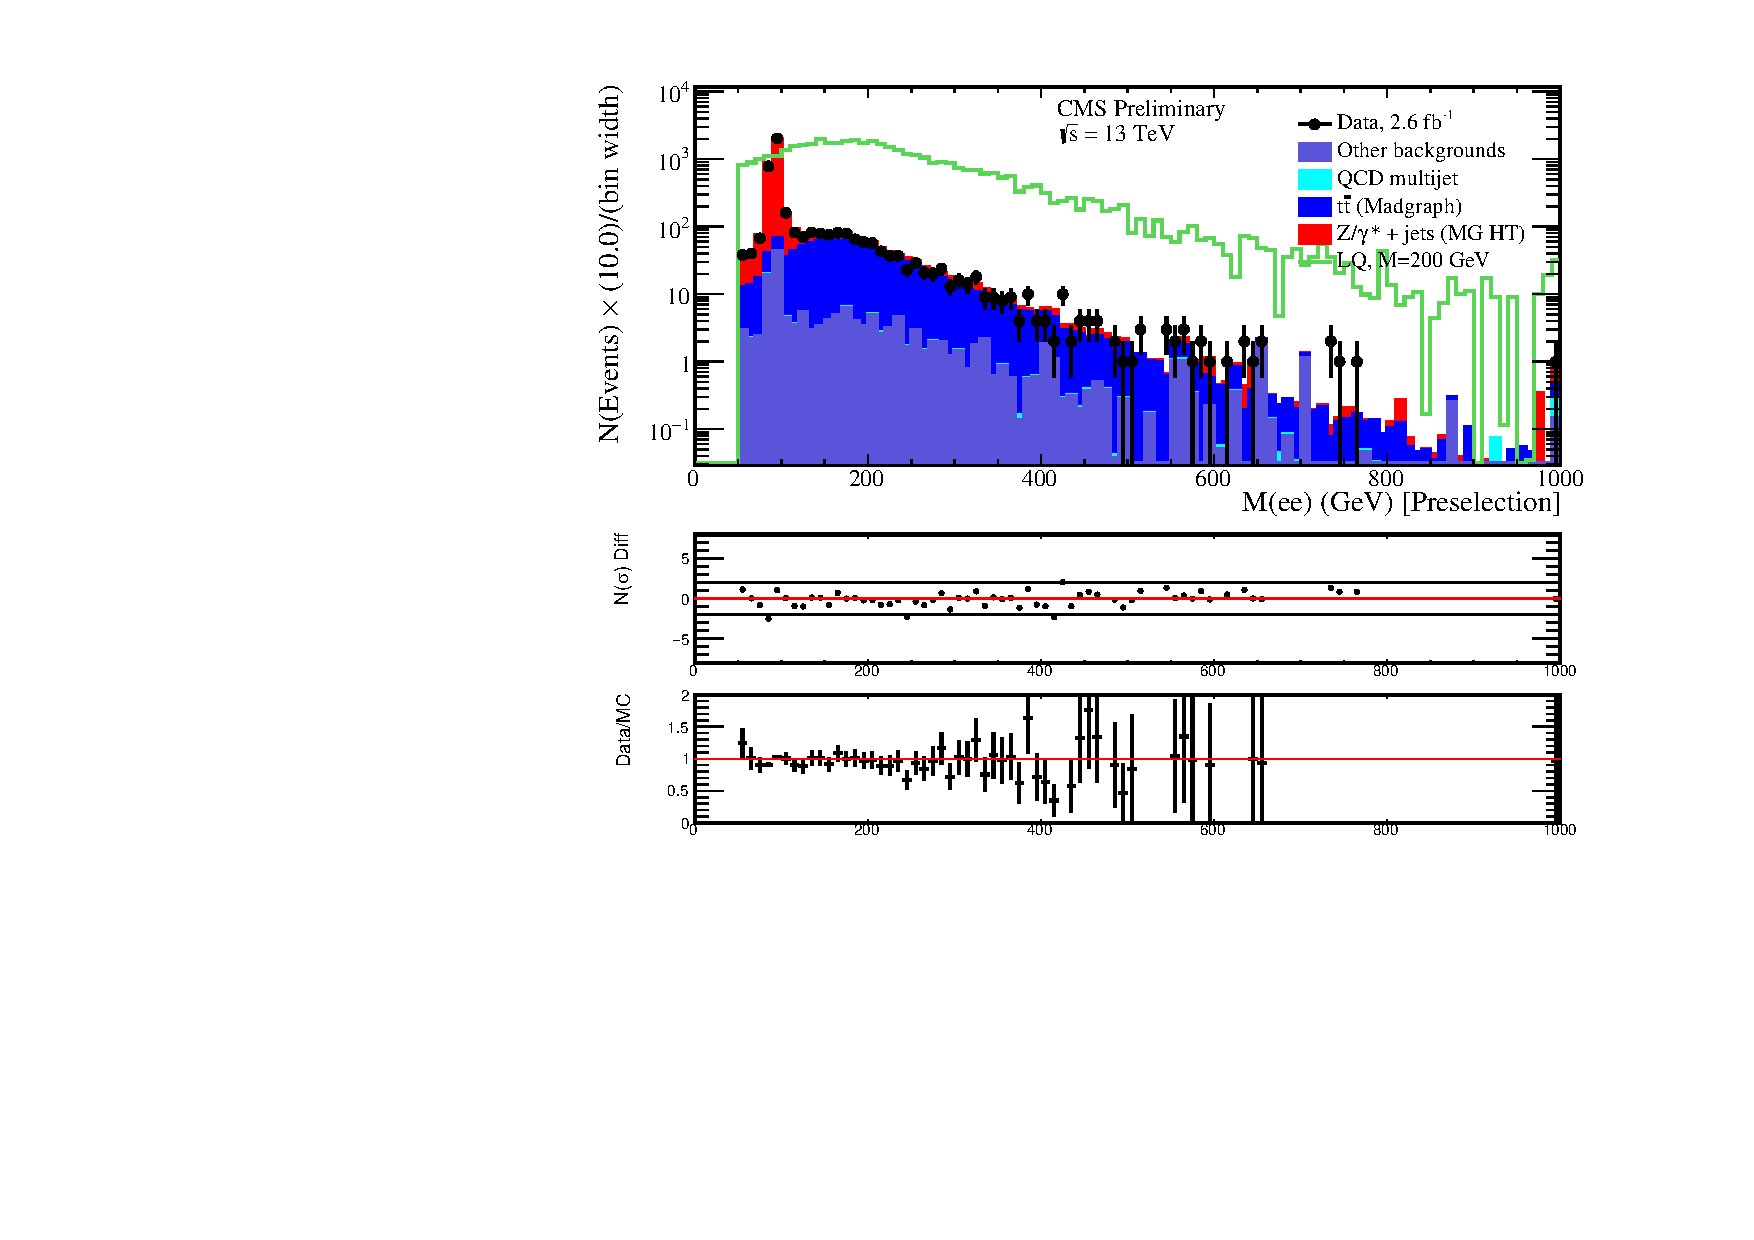
\includegraphics[width=0.32\textwidth]{/home/bibhu/Desktop/PhDThesis/PhDThesis/synopsis/Mee_PAS_eejj.pdf}
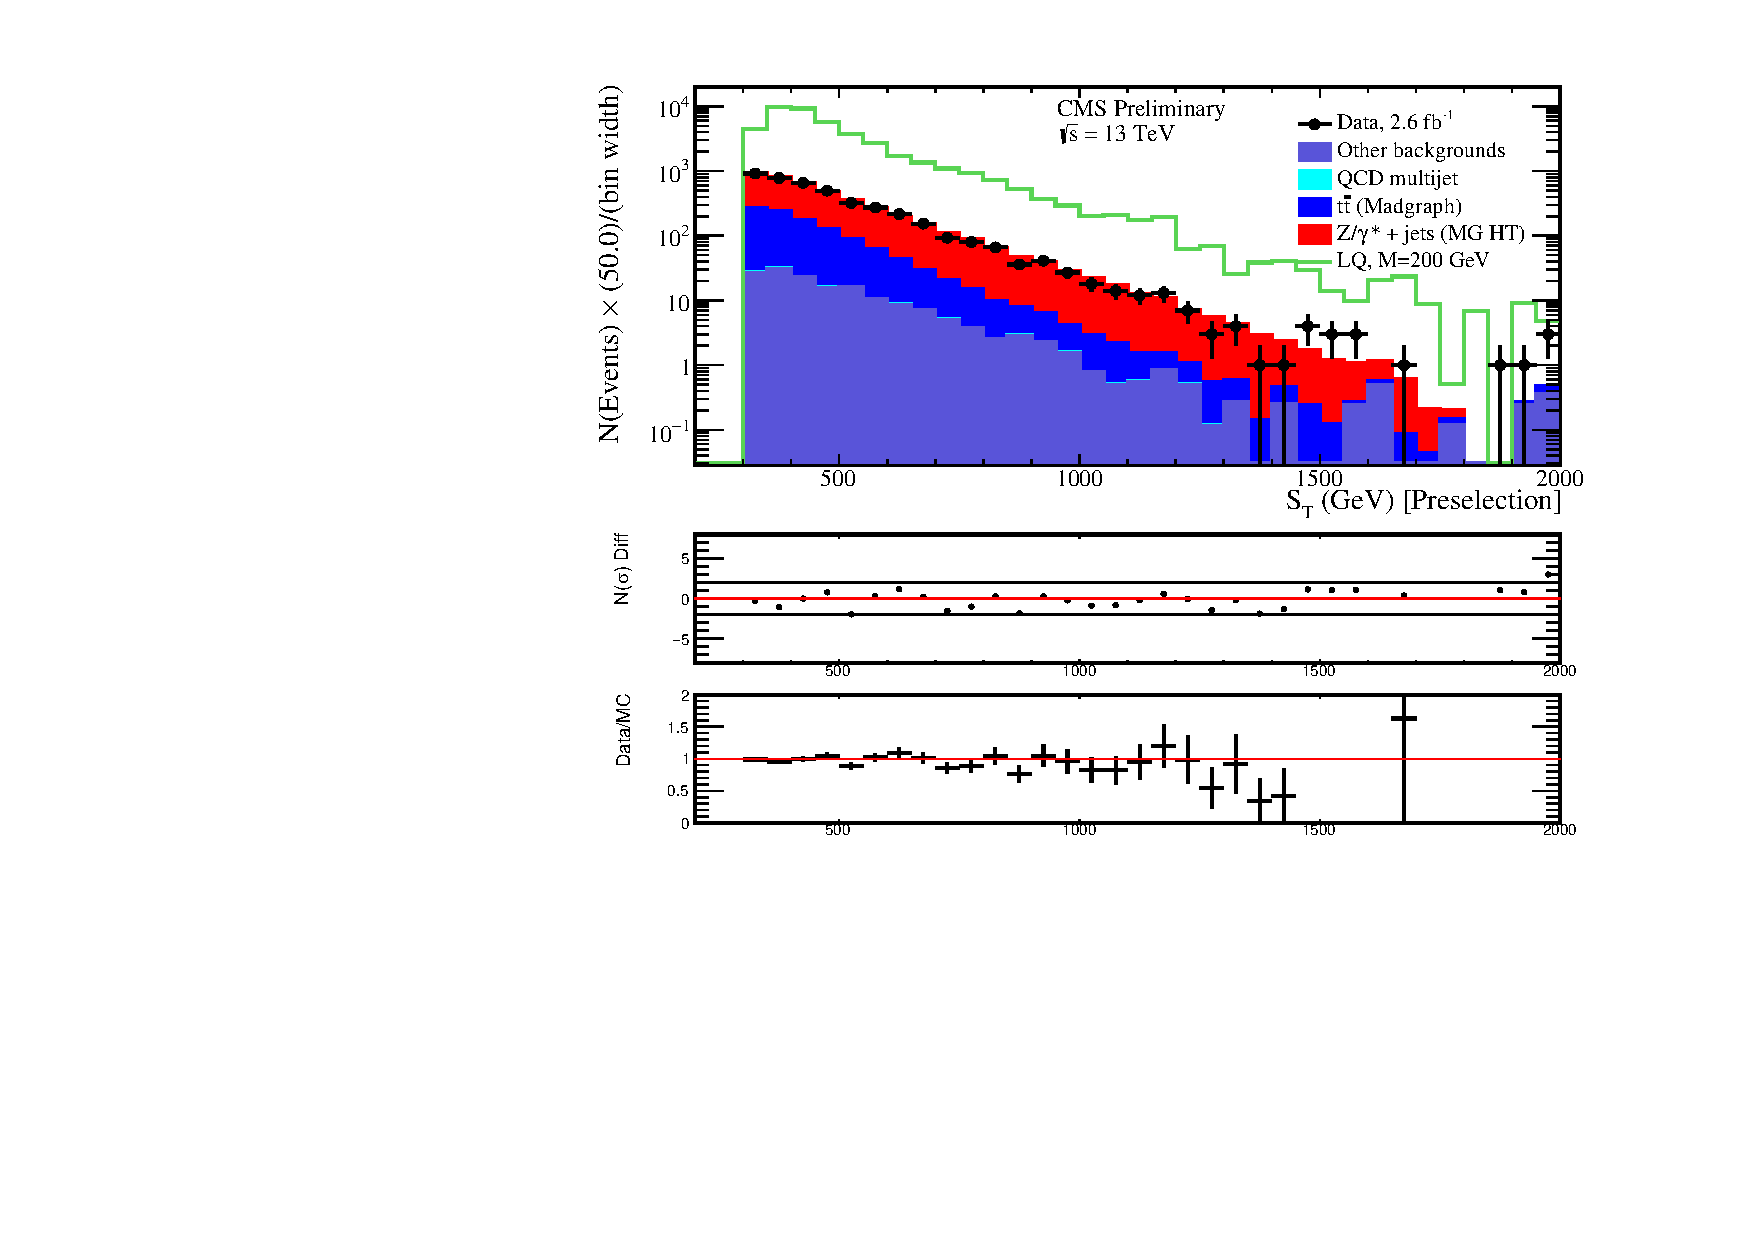
\includegraphics[width=0.32\textwidth]{/home/bibhu/Desktop/PhDThesis/PhDThesis/synopsis/sT_PAS_eejj.pdf}
\caption{\label{figure:DataVsMCinVariableLQ1}Data vs. background plots for $\rm M_{ee}$ (left) and $\rm S_{T}$ (right). }
\end{figure}


\subsection{Background Estimation}

The major backgrounds from SM processes are Z+jets and $\rm t\bar{t}$, where single top,
 W+jets, diboson, and $\gamma$+jets contribute at a lower level. There is also an instrumental background from QCD events with jets faking electrons. Below we describe how these
backgrounds are determined in our analysis.
\begin{itemize}
\item The Z+jets and $\rm t\bar{t}$ background shapes are taken from MC simulations, and normalized
 to data using the eejj preselection. More details are given in Ref.~\cite{CMS-PAS-EXO-16-043}.
\item Single top, W+jets, diboson, and $\gamma$+jets backgrounds are derived completely from
 MC samples that are scaled to the cross sections.
 \item QCD background is determined using a data-driven fake rate method, as
 described in Ref.~\cite{CMS-PAS-EXO-16-043}.

\end{itemize}




\subsection{Results}
Similar to the two SUSY analyses, we observe no significant excess of events as compared to the SM backgrounds. The broad excess of the events that was seen in the 8 TeV analysis~\cite{CMS-PAS-EXO-12-041} has disappeared with the 2015 data. We set the upper limits on the cross section times branching fraction using the same tool as before. Fig. ~\ref{figure:LimitLQ12016Synop} shows both the observed and expected limits for different leptoquark masses. We exclude leptoquark masses up to 1130 GeV from this study. 

\begin{figure}[h]
\centering
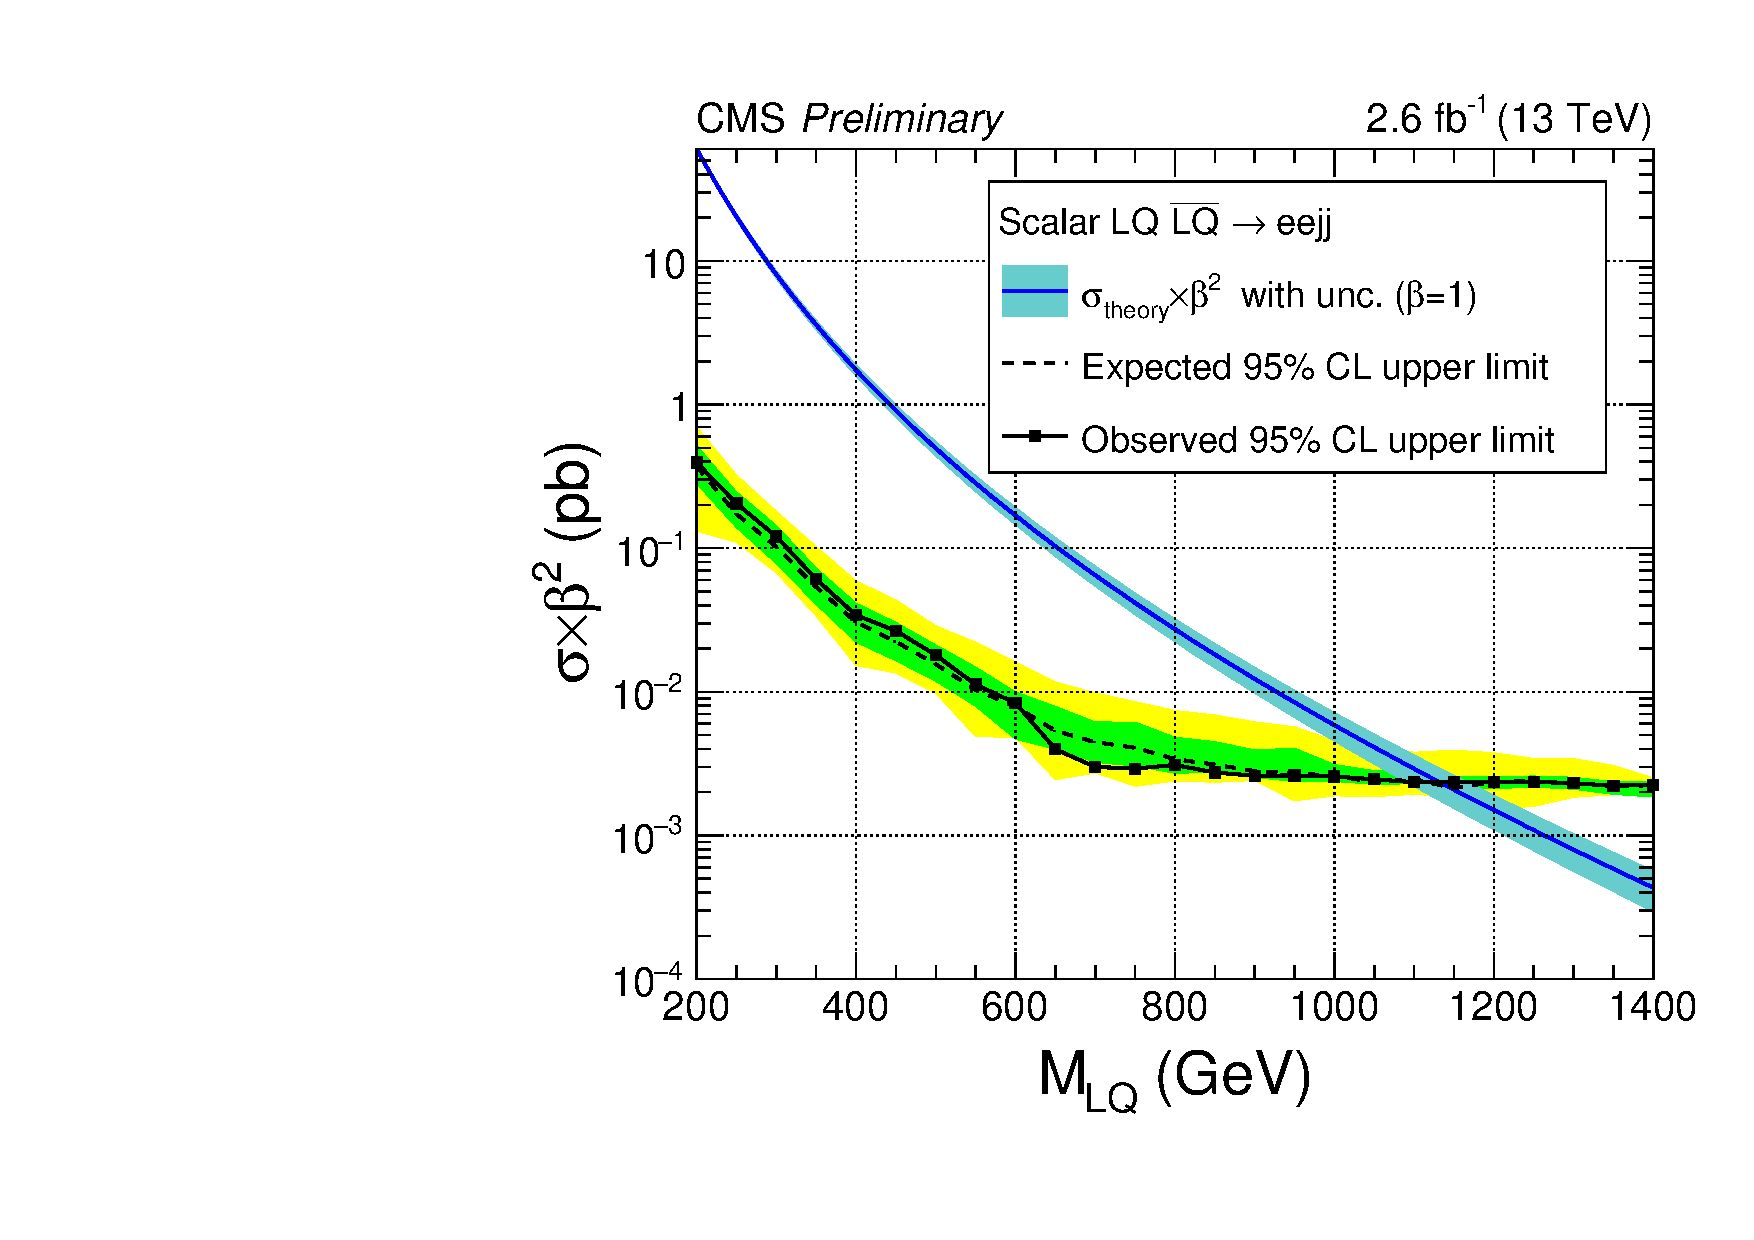
\includegraphics[width=0.32\textwidth]{/home/bibhu/Desktop/PhDThesis/PhDThesis/synopsis/LQLimitPlot.pdf}

\caption{\label{figure:LimitLQ12016Synop}The 95\% CL upper limits on the production cross sections as a function of leptoquark mass.}
\end{figure}



\section{Advanced Pileup Mitigation Techniques}

\subsection{Jet Grooming }
Grooming, introduced in Ref.~\cite{Grooming}, is intended to remove soft and wide-angle radiation from a jet.  
It is typically used to reduce the overall jet mass of QCD (quark- and gluon-initiated) jets while retaining the larger jet mass for jets originating from heavy particles such as the top quark and W/Z/H boson. Additionally, it can also help minimize the pileup dependence on jet mass. In general, grooming alters the soft structure of the jet while other observables may rely on this soft structure. Here we explore three grooming methods to mitigate the effects of pileup on large-R jets (R=0.8).


{\bf 1. }Pruning ~\cite{Ellis:2009me} reclusters the constituents of the jet through the Cambridge-Aachen (CA) algorithm ~\cite{Dasgupta:2013ihk} using the same distance parameter.  
At each step in the clustering algorithm, the softer of the two particles $i$ and $j$ to be merged is removed when the following conditions are met:
 

$z_{ij} = \frac{{\rm min}(\rm p_{T_{i}}, p_{T_{j}})}{\rm p_{T_{i}} + p_{T_{j}}} < z_{\rm cut}$ and 
$\Delta R_{ij} >  \frac{2 \times r_{\rm cut} \times m_{J}}{\rm p_{T}} $,

where $m_{J}$ and $\rm p_{T}$ are the mass and transverse momentum of the originally-clustered jet, and $z_{\rm cut}$ and $r_{\rm cut}$ are parameters of the algorithm.

{\bf 2. }Trimming ~\cite{Krohn:2009th} ignores particles within a jet that fall below a dynamic threshold in $\rm p_{T}$. 
It reclusters the constituents of the jet using the $\rm k_{t}$ algorithm ~\cite{Cacciari:2008gp} with a radius parameter $r_{\rm sub}$, accepting only the subjets that have $\rm p_{T_{\rm sub}} > p_{Tfrac} \lambda_{\rm hard}$, where $\rm p_{Tfrac}$ is a dimensionless cutoff parameter, and $\lambda_{\rm hard}$ is some hard QCD scale chosen to be equal the $\rm p_{T}$ of the original jet. 

{\bf 3. }Soft-drop ~\cite{Larkoski:2014wba}  declusters the jet recursively to remove soft and wide-angle radiation from the jet.
The jet is reclustered using the CA algorithm.  Then the jet is declustered and at each step, subjets $j_{1}$ and $j_{2}$ are used to define the following condition:

$\frac{{\rm min}(\rm p_{T_{j1}},\rm p_{T_{j2}})}{\rm p_{T_{j1}}+p_{T_{j2}}} > z_{\rm cut} \times \left( \frac{\Delta R_{12}}{R_0} \right)^{\beta}$

where the algorithm parameters are $z_{\rm cut}$ and $\beta$.
If the condition is met, the declustering continues, otherwise only the leading $\rm p_{T}$ subjet is kept.
In the case when $\beta=0$, soft drop can be considered a generalization of the modified mass drop tagger (MMDT)~\cite{Dasgupta:2013ihk}. 


The (groomed) masses are corrected for pileup using a four-vector safe subtraction. %~\cite{Cacciari:2014jta}.
In the cases of soft drop and trimming, the four-vector subtraction corrects the jet $\rm p_{T}$ and mass at each step in the algorithm.
For pruning, however, the correction is applied to the final product using the pruned jet area. 
The parameters for the grooming algorithms explored in this study can be found in Ref.~\cite{JMEPAS} % Table~\ref{tab:groom}.

%\begin{table}[ht]
%\begin{center}
%\begin{tabular}{|c|c|}
%    \hline
%    Grooming algorithm & Parameters \\
%    \hline
%    \hline    
%    \multirow{4}{*}{Pruning} & $z_{\rm cut}$ = 0.1, $r_{\rm cut}$ = 0.5\\
%    & $z_{\rm cut}$ = 0.05, $r_{\rm cut}$ = 0.5\\
%    & $z_{\rm cut}$ = 0.1, $r_{\rm cut}$ = 0.75\\
%    & $z_{\rm cut}$ = 0.05, $r_{\rm cut}$ = 0.75\\        
%    \hline
%    \multirow{4}{*}{Trimming} & $r_{\rm sub}$ = 0.2, \pt$_{\rm frac}$ = 0.05\\
%    & $r_{\rm sub}$ = 0.2, \pt$_{\rm frac}$ = 0.03\\    
%    & $r_{\rm sub}$ = 0.1, \pt$_{\rm frac}$ = 0.03\\    
 %   & $r_{\rm sub}$ = 0.3, \pt$_{\rm frac}$ = 0.03\\            
%    \hline
%    \multirow{4}{*}{Soft drop/MMDT} & $z_{\rm cut}$ = 0.1, $\beta$  = 0 \\
%     & $z_{\rm cut}$ = 0.1, $\beta$  = 1 \\    
%     & $z_{\rm cut}$ = 0.1, $\beta$  = 2 \\    
                  
%    \hline    
%\end{tabular}
%\caption{Summary of grooming parameters
%\label{tab:groom}}
%\end{center}
%\end{table}



\subsection{Results}

\begin{figure}[h]
\centering
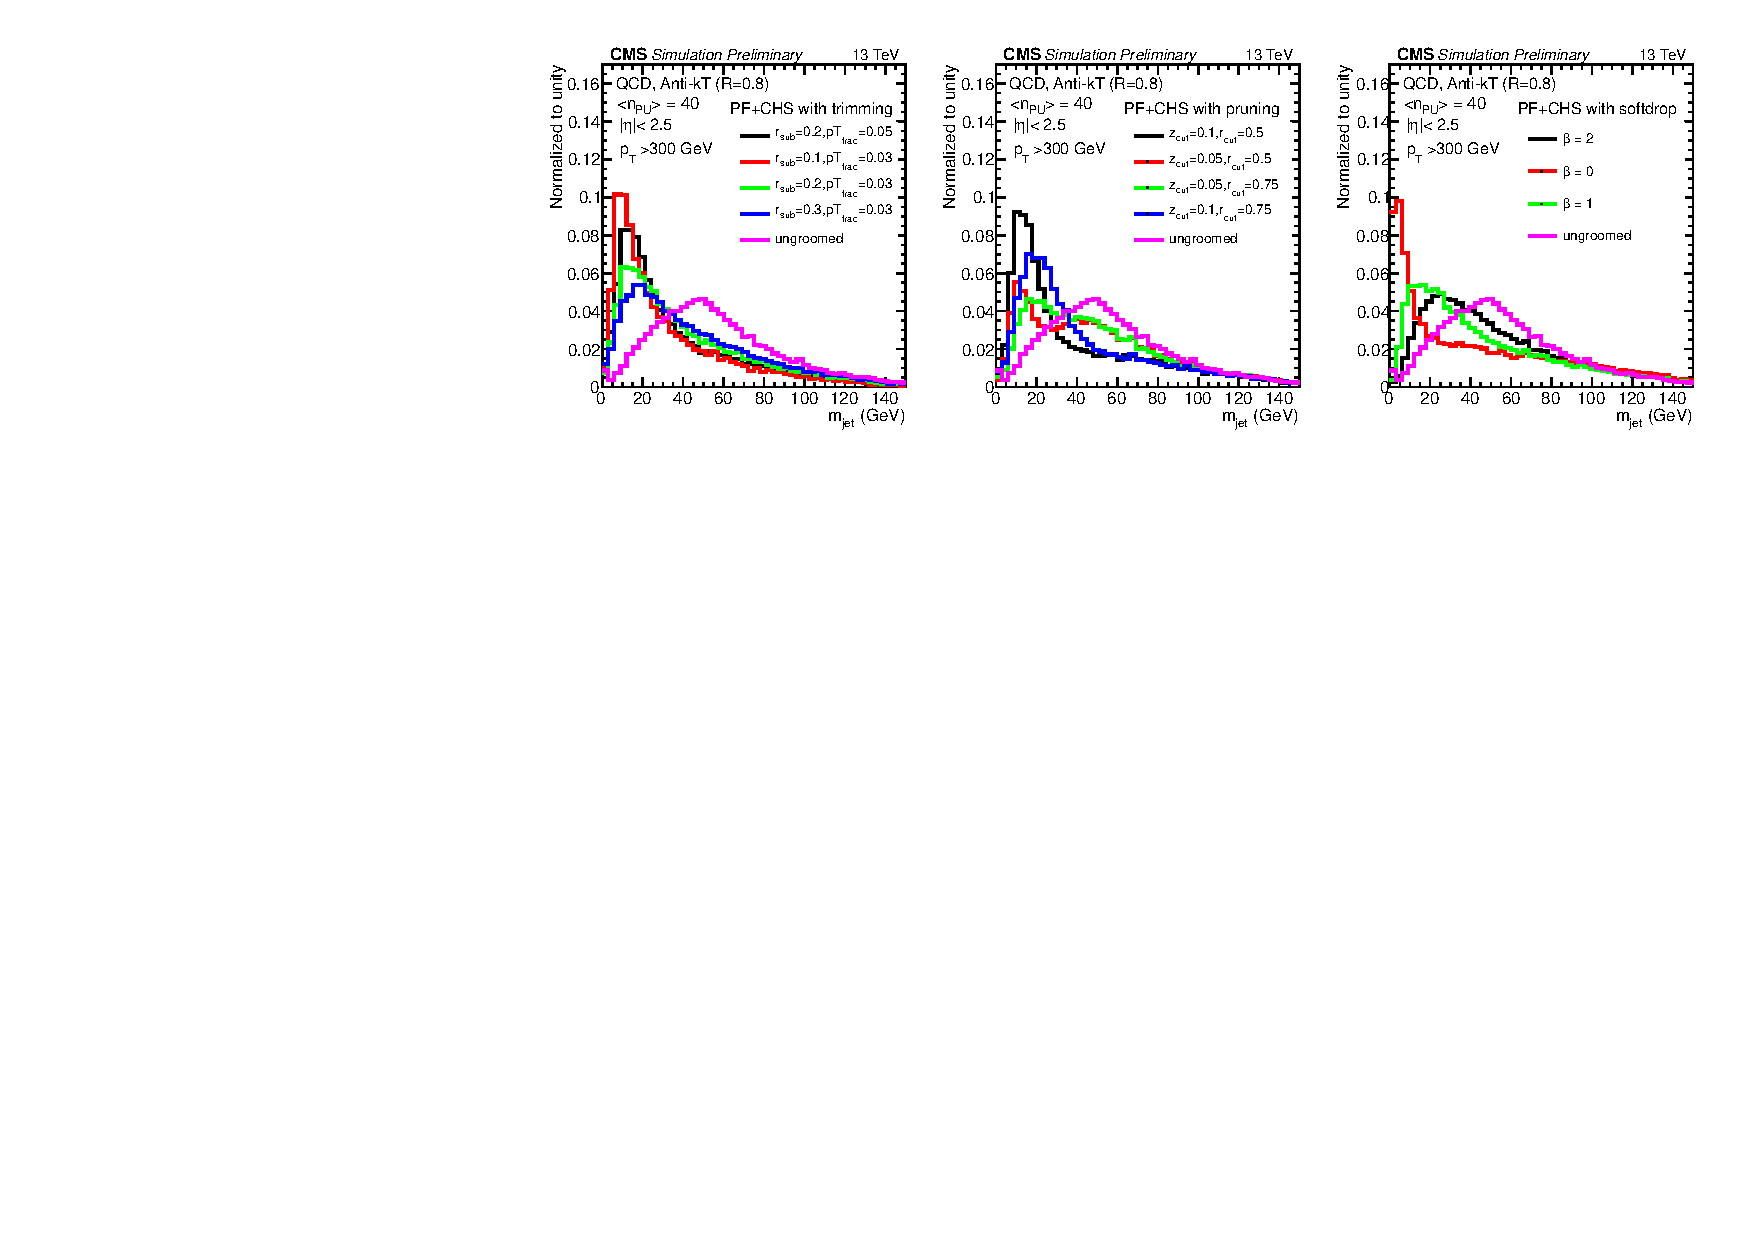
\includegraphics[width=15cm,height=5cm]{/home/bibhu/Desktop/PhDThesis/PhDThesis/synopsis/1DPFCHS_QCD.pdf}

\caption{\label{fig:grooming1D} The mass distributions of PFCHS jets after application of trimming (left), pruning (middle) and soft-drop (right) for different set of parameters. The ungroomed mass distribution is shown to compare the aggressiveness of grooming methods. }
\end{figure}

\begin{figure}[h]
\centering
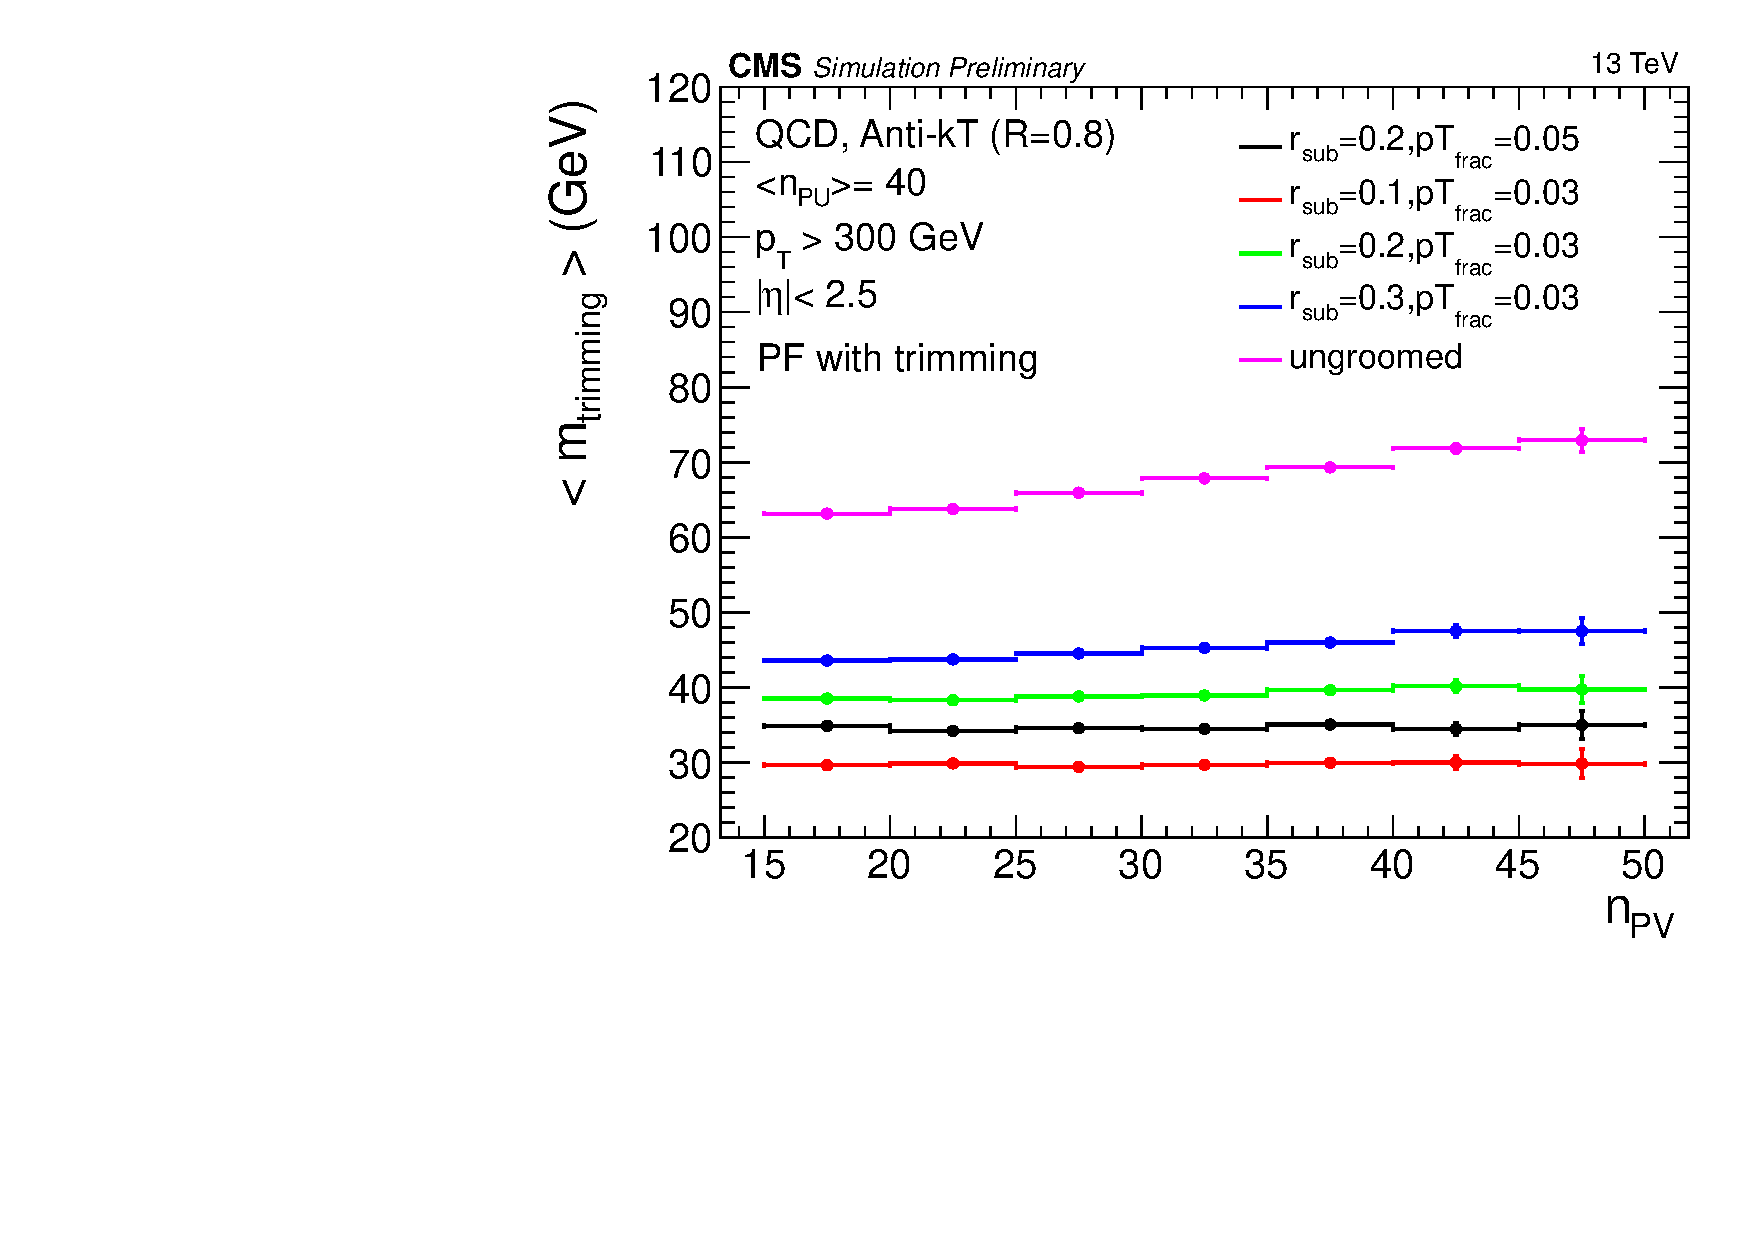
\includegraphics[width=0.3\textwidth]{/home/bibhu/Desktop/PhDThesis/PhDThesis/synopsis/AvJetmass_Vs_nPV_PF_trim.pdf}
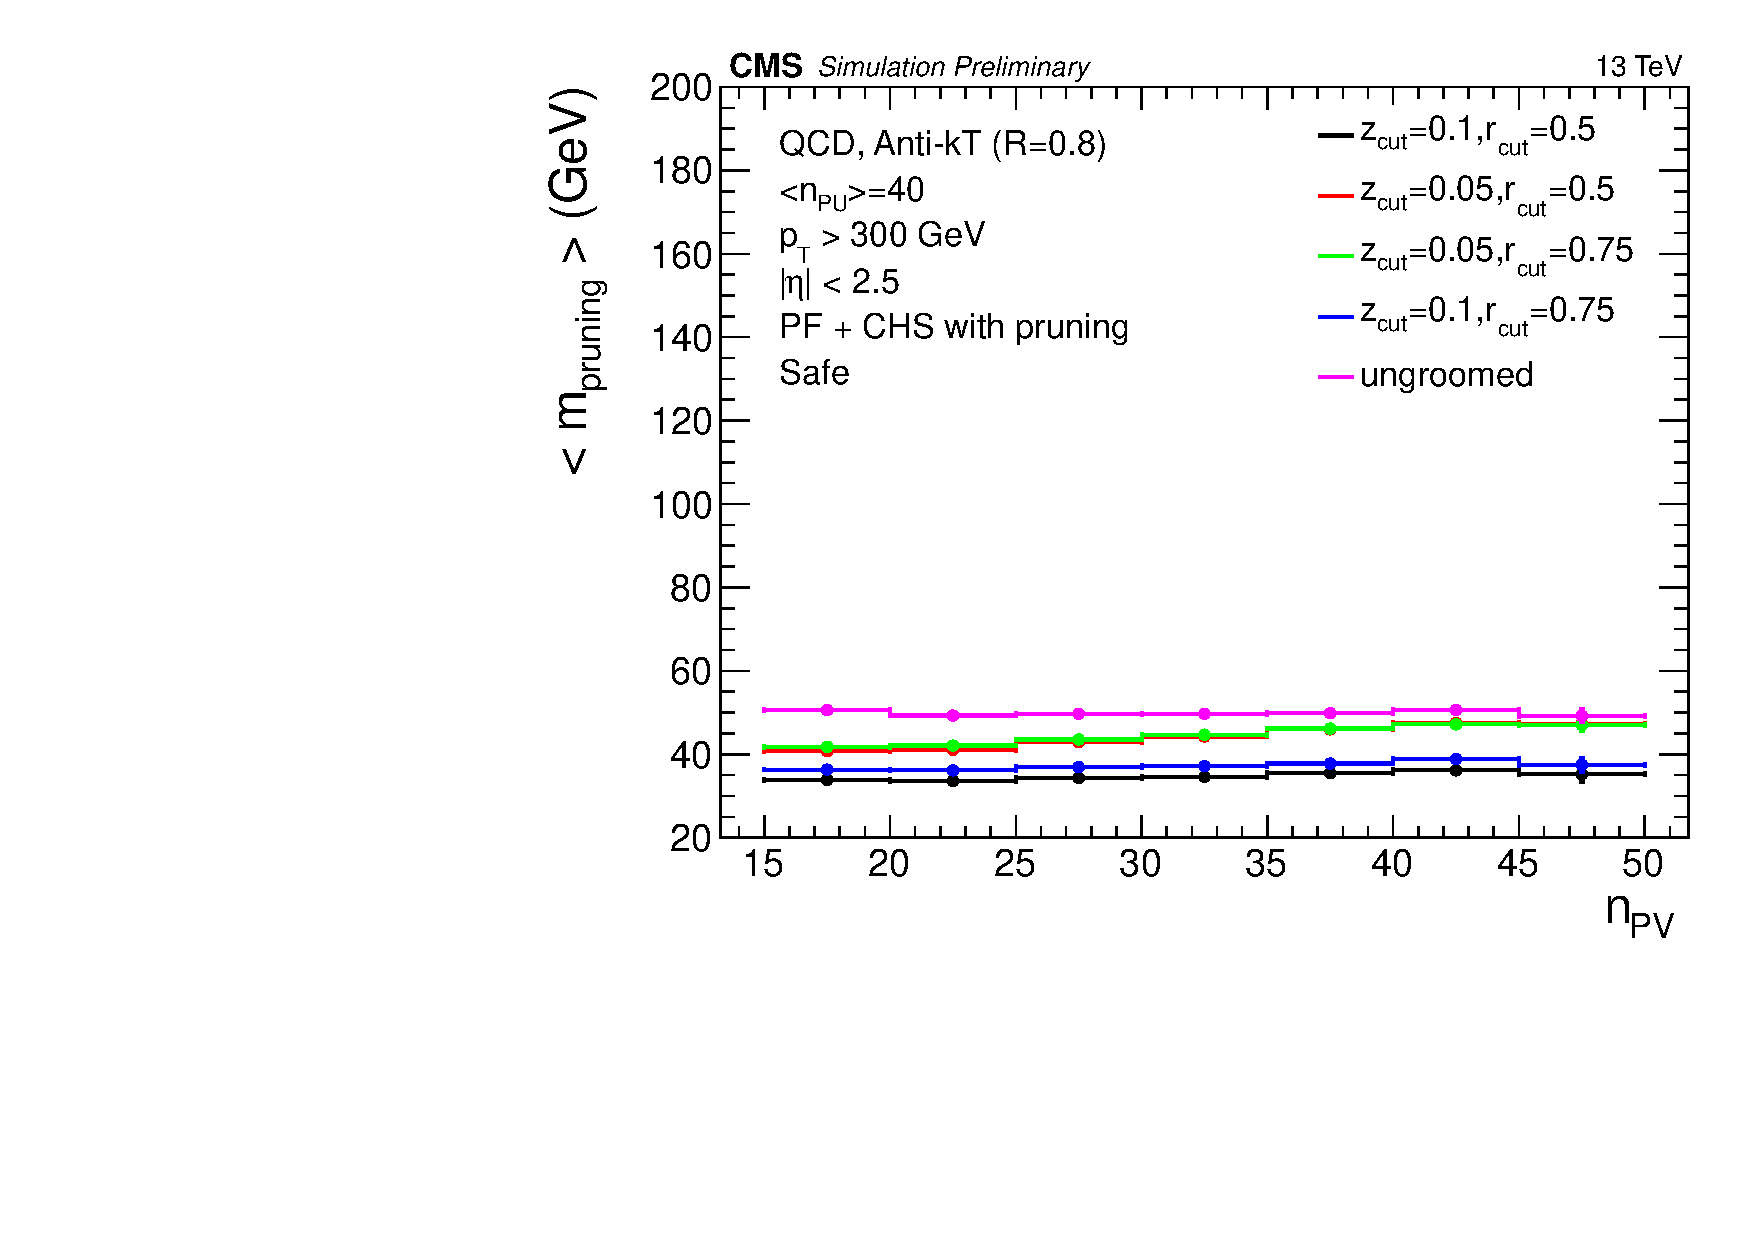
\includegraphics[width=0.3\textwidth]{/home/bibhu/Desktop/PhDThesis/PhDThesis/synopsis/AvJetmassSafe_PFCHS_prun.pdf}
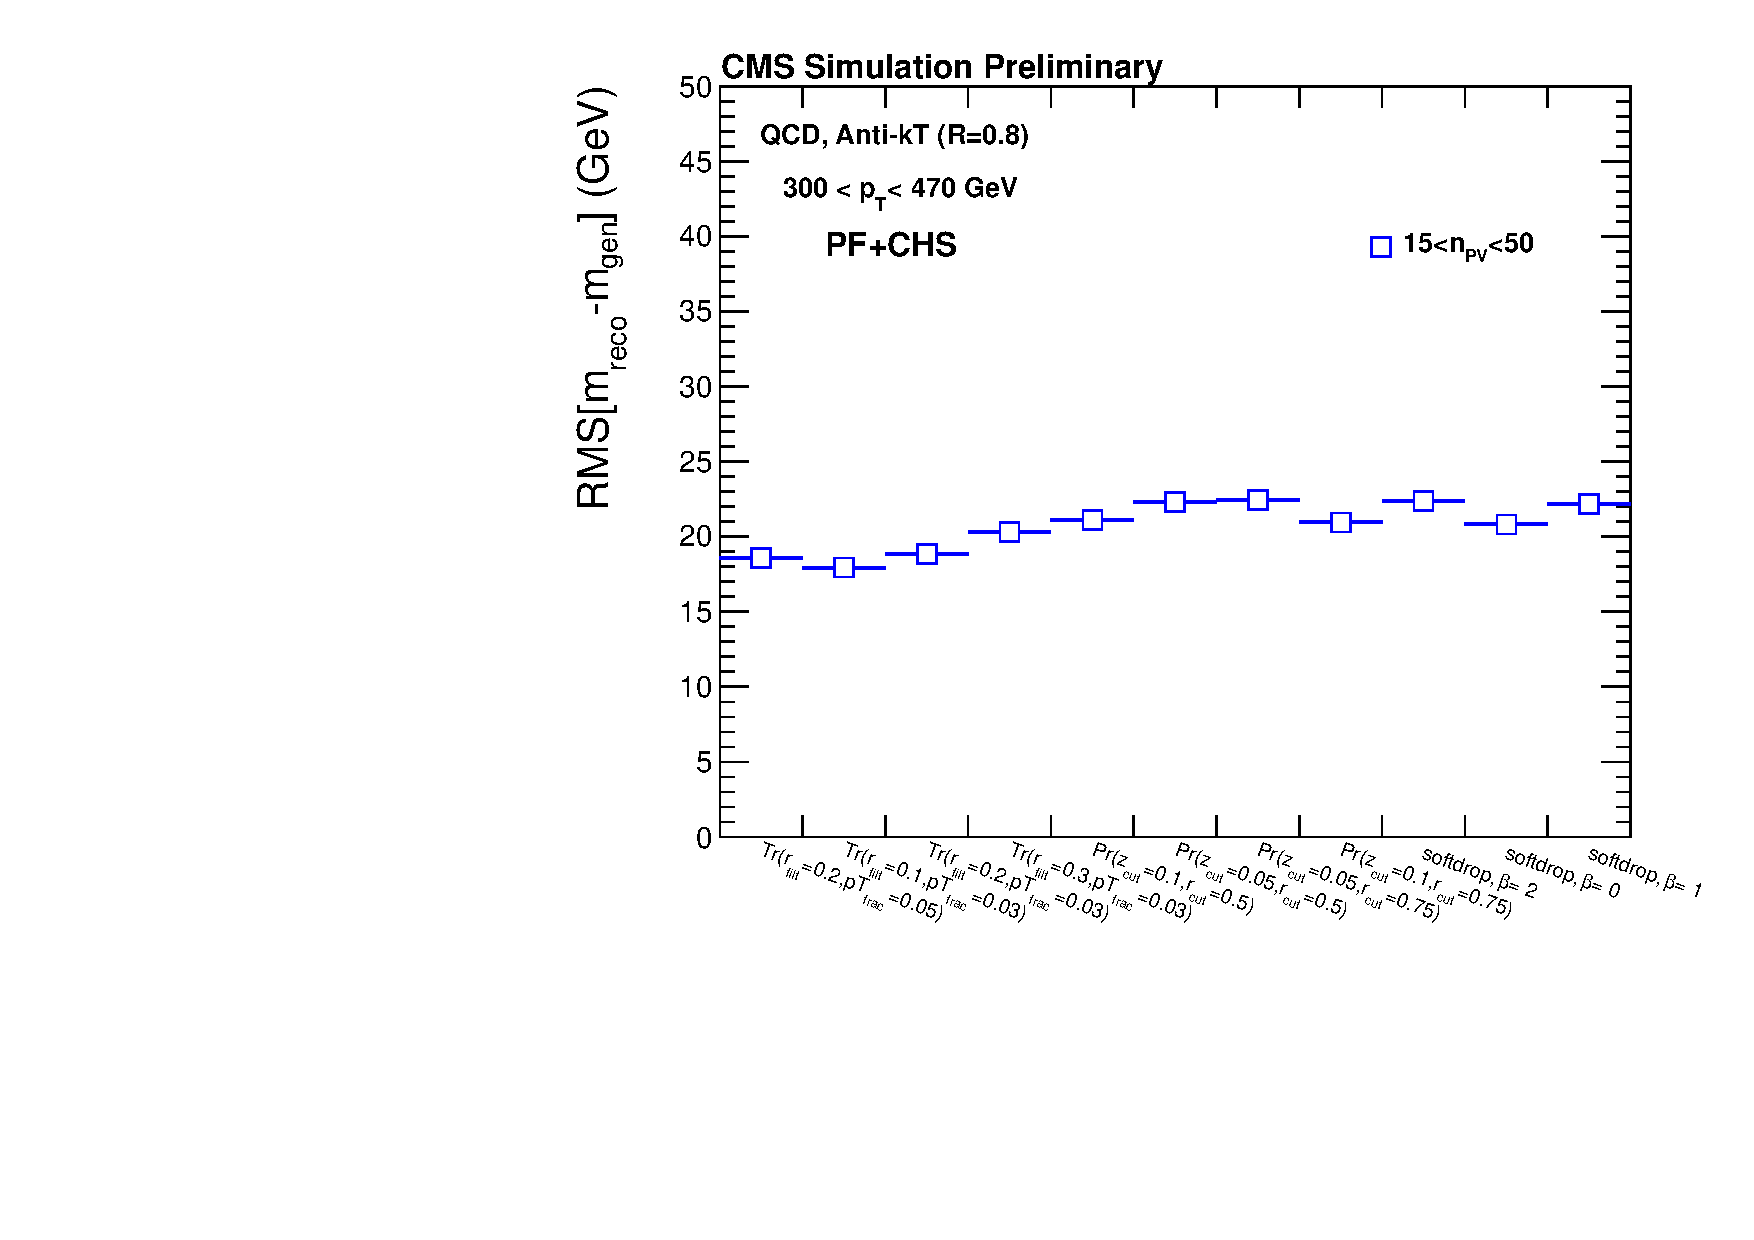
\includegraphics[width=0.3\textwidth]{/home/bibhu/Desktop/PhDThesis/PhDThesis/synopsis/SummaryPFCHSallNPV.pdf}
\caption{\label{fig:Groom}Variation of average jet mass vs. number of primary vertices for trimming (left), pruning (middle) and RMS in various grooming techniques (right).  }
\end{figure}

The groomed mass distributions of charged hadron subtracted PF (PFCHS) ~\cite{Beaudette:2014cea, JMEPAS} jets are shown in Fig.~\ref{fig:grooming1D}. One sees that after the application of grooming due to the reduction of pileup the peaks in the distributions shift to left whereas in the ungroomed case they have an unphysical looking like peak in the higher side. Even though these mass distributions do not tell everything but they say because of the application of grooming the mass distributions change aggressively.  

Average jet mass and jet resolutions are taken as quality parameters for determining the robustness of pileup mitigation algorithms. The plots of average jet mass vs. the number of primary vertices are shown in Fig.~\ref{fig:Groom}. The left plot shows the average jet mass is stable for trimmed jets but not for ungroomed jets. However, once the charged hadron subtraction is applied jet mass becomes stable considerably that can be seen from the middle plot. The right plot summarizes the results in terms of jet mass resolution from three different grooming techniques considered here.


\section{Summary}

We have presented the searches for SUSY and leptoquarks with 13 TeV pp collision data recorded with CMS. The SUSY search targets for direct gluino, stop and squark pair production in all hadronic final state. Two separate searches with 2.3 $\rm fb^{-1}$ of 2015 and 12.9 $\rm fb^{-1}$ of 2016 data yield null results of new physics. Similarly no signatures of any signal are found in the search of  first generation scalar leptoquarks performed with 2.6 $\rm fb^{-1}$ of the 2015 data. Upper limits on the signal cross section  are obtained in all three cases significantly extending the previous 8TeV limits.   

Lastly, a study on advanced pileup mitigation techniques is presented. Performance of various jet grooming methods like trimming, pruning and soft-drop are compared. Optimized quality parameters of these techniques are recommended for future use.   


%\begin{table}
%\centering
%\begin{tabular}{l|r}
%Item & Quantity \\\hline
%Widgets & 42 \\
%Gadgets & 13
%\end{tabular}
%\caption{\label{tab:widgets}An example table.}
%\end{table}

\newpage

%\bibliography{Synopsis.bib}
%\bibliographystyle{utphys.bst}








\clearpage






